\newpage
\chapter{Фрактальные квадраты с конечным пересечением}


\section{Пересечения копий фрактального квадрата}


\subsection{Фрактальные квадраты}

\begin{definition}\label{dfn:FS} 
Пусть $D=\{d_1,\ldots,d_m\}\IN\{0,1,\ldots,n-1\}^2$, где $n\ge 2$, и $1<m<n^2$.
{\em Фрактальным квадратом} порядка $n$ с {\em множеством единиц $D$} называют компактное множество $K\IN\rr^2$, удовлетворяющее уравнению
\begin{equation}\label{fsqeq}
K=\dfrac{K+D}{n}.
\end{equation}
\end{definition}

Уравнение \eqref{fsqeq} можно будет использовать в его эквивалентной форме $nK=K+D$.
Само же множество $K$ содержится в $P$, поскольку единичный квадрат $P=[0,1]^2$ удовлетворяет уравнению $nP\NI P+D$

\begin{figure}[H]
 \centering
 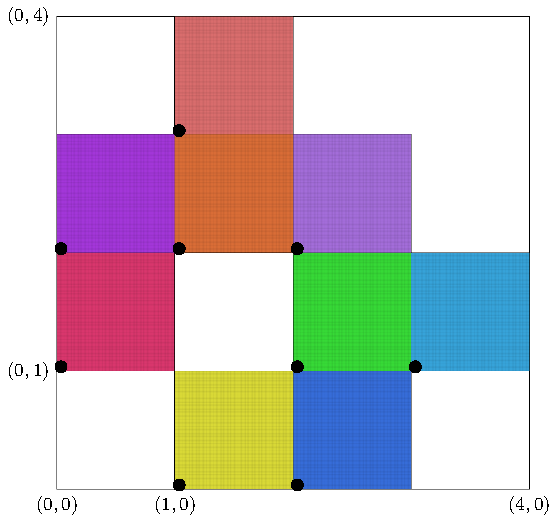
\includegraphics[width=0.48\textwidth]{digitset.pdf}
 \hfill
 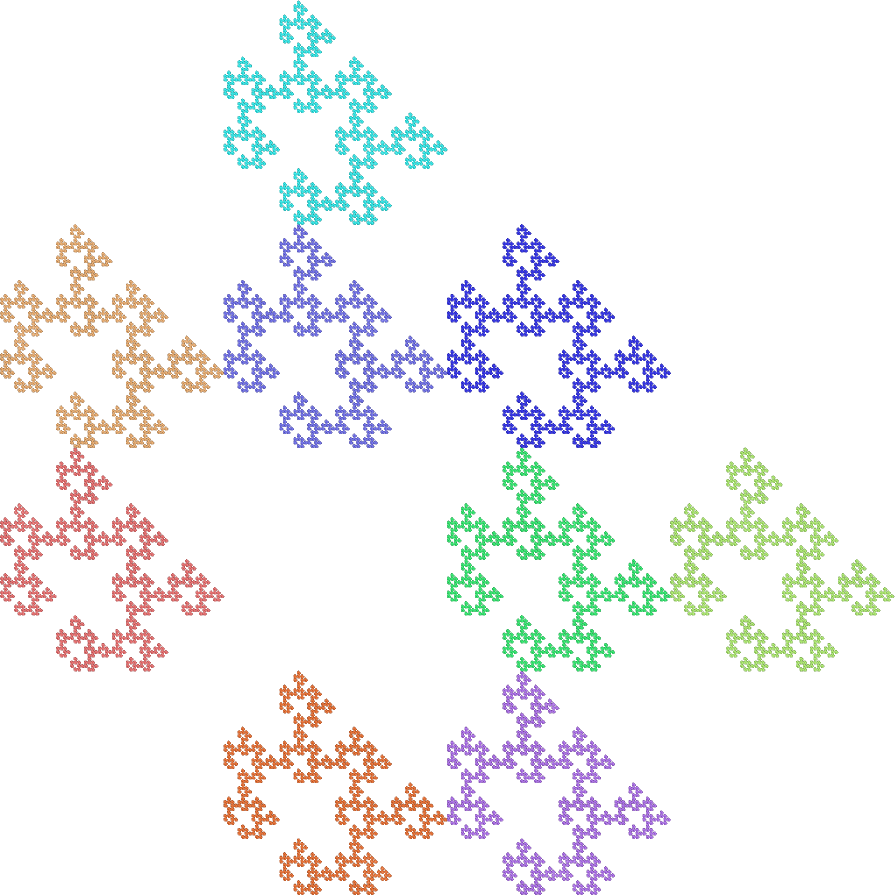
\includegraphics[width=0.42\textwidth]{den2f.png}
 \caption{Множество $n(D+P)$ (слева) и фрактальный квадрат $nK=K+D$ (справа). Элементы из $D$ отмечены чёрными точками.}
 \label{fig:fr_sq}
\end{figure}

Мы можем рассмореть единичный квадрат $P$ и разбить его вертикальными и горизонтальными отрезками на $n^2$ маленьких квадратов с ребром $1/n$.
Из этого разбиения выберем некоторые квадраты.
Нижний левый угол каждого выбранного квадрата имеет координату вида $\dfrac{d_i}{n}$, где $d_i\in\{0,1,\ldots,n-1\}^2$ --- единица из множесва единиц $D$.
Значит гомотетия, переводящая единичный квадрат $P$ в маленький квадрат квадрат с координатами нижнего левого угла $\dfrac{d_i}{n}$, имеет вид $S_i(x)=\dfrac{x+d_i}{n}$.

Уравнение \eqref{fsqeq} определяет систему $\eS$ гомотетий $S_i(x)=\dfrac{x+d_i}{n}$, где $d_i\in D$, а оператор Хатчинсона $T_\eS$ системы $\eS$ определяется уравнением $T_\eS(A)=\dfrac{D+A}{n}=\bigcup\limits_{d_i\in D}\dfrac{d_i+A}{n}$.

\begin{definition}\label{refin}
 Для любого $k\in \nn$, {\em $k$-е измельчение} системы $\eS$ --- это система $\eS^k=\{S_\bi, \bi=i_1i_2\ldots i_k\in I^k\}$, где $S_\bi(x)=\dfrac{x+d_\bi}{n^k}$ и $d_\bi=n^{k-1}d_{i_1}+n^{k-2}d_{i_2}+\ldots+d_{i_k}$. 
\end{definition}

Сисиема $\eS^k$ представляет $K$ как фрактальный квадрат порядка $n^k$ с множеством единиц $D^k=n^{k-1}D+n^{k-2}D+\ldots+D$ и копиями $\dfrac{K+d_\bi}{n^k}$.
Оператор Хатчинсона $T_\eS^k$ этой системы $\eS^k$ определяется уравнением $T_\eS^k(A)=\dfrac{D^k+A}{n^k}$.

Каждой бесконечной строке $\bi=i_1i_2\ldots\in I^\8$ соответствует единственная точка $x=\pi(\bi)$ по формуле $\pi(\bi)=\sum\limits_{k=1}^\8 \dfrac{d_{i_k}}{n^k}$.

\begin{remark}% \label{rmk:fsd}
Далее, если не указано иное, говоря {\em <<фрактальный квадрат $K$>>}, мы будем иметь ввиду {\em <<фрактальный квадрат $K$ порядка $n$ множеством единиц $D$>>}. 
\end{remark}


\subsection{Грани $K_\al$ и пересечения граней $F_\al$ фрактального квадрата}

Поскольку фрактальный квадрат $K=K(\eS)$ содержится в единичном квадрате $P$, то $S_i(K)\IN S_i(P)$ для любого $S_i\in\eS$.
Тогда для любых $S_i, S_j\in\eS$ маленькие квадраты $S_i(P)$ и $S_j(P)$ если и пересекаются друг с другом, то пересекаются по своим граням, соответствующие праобразы которых относительно отображений $S_i$ и $S_j$ являются парой противоположных граней в квадрате $P$.
Значит нам нужно обозначить крани квадрата $P$ и лежащие в этих гранях точки из фрактального куба $K$.


\begin{definition}\label{setA}
Обозначим как $A=\{-1,0,1\}^2$ множество векторов $\bma=(\al_1,\al_2)$. 
\end{definition}

Между множеством $A$ и множеством граней единичного квадрата $P=[0,1]^2$ существует взаимно-однозначное соответствие:

\begin{definition}\label{dfn:Pa}
Каждый вектор $\bma\in A=\{-1,0,1\}^2$ задаёт единственную грань $P_\bma$ единичного квадрата $P$ равенством $P_\bma=P\cap(P+\bma)$.
\end{definition}

Симметрия противоположных граней квадрата $P$ выражается равенством 
$$P_\bma=P\cap(P+\bma)=((P-\bma)\cap P)+\bma=P_{-\bma}+\bma.$$


Существует отношение порядка $\sqsubseteq$ на $A$, которое изоморфно отношению включения $\supseteq$ граней куба $P$.
%\red{There is an order relation $\sqsubseteq$ on the set $A$ which is order isomorphic to the inclusion ordering $\supseteq$ of the faces of $P$.}

\begin{definition}\label{Aorder}
Пусть $\bma=(\al_1,\al_2)$, $\bmb=(\be_1,\be_2)\in A$, тогда говорим, что $\bma\sqsubseteq\bmb$, если для $\al_i\neq 0$ верно $\be_i=\al_i$.
% , and $\al_i= 0$ implies $\be_i\neq 0$. 
Если при этом $\bma\neq\bmb$ тогда говорим, что $\bma\sqsubset\bmb$.
\end{definition}

Очевидно, что $\bma\sqsubseteq\bmb$ если и только если $P_\bma\supseteq P_\bmb$. 
Максимальными элементами из $A$ по отношению $\sqsubseteq$ являются $(\pm 1,\pm 1)$, поэтому грани $P_{(-1,-1)}, P_{(1,-1)}, P_{(-1,1)}, P_{(1,1)}$ соответствуют угловым точкам $(0,0), (1,0), (0,1), (1,1)$ квадрата $P$.
Минимальным элементом из $A$ по отношению $\sqsubseteq$ является $(0,0)$, которому соответствует единичный квадрат $P=P_{(0,0)}$.

\begin{definition}\label{def-falpha}
Гранью $K_\bma$ фрактального квадрата $K$ называется пересечение $K\cap P_\bma$.
Пересечением $F_\bma$ мы называем пересечение $K_\bma\cap(K_{-\bma}+\bma)$ пары противоположных граней фрактального квадрата.
\end{definition}



\begin{figure}[H]
 \centering
 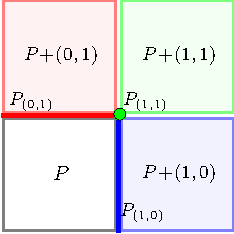
\includegraphics[width=0.45\textwidth]{faces_p.pdf}
 \hfill
 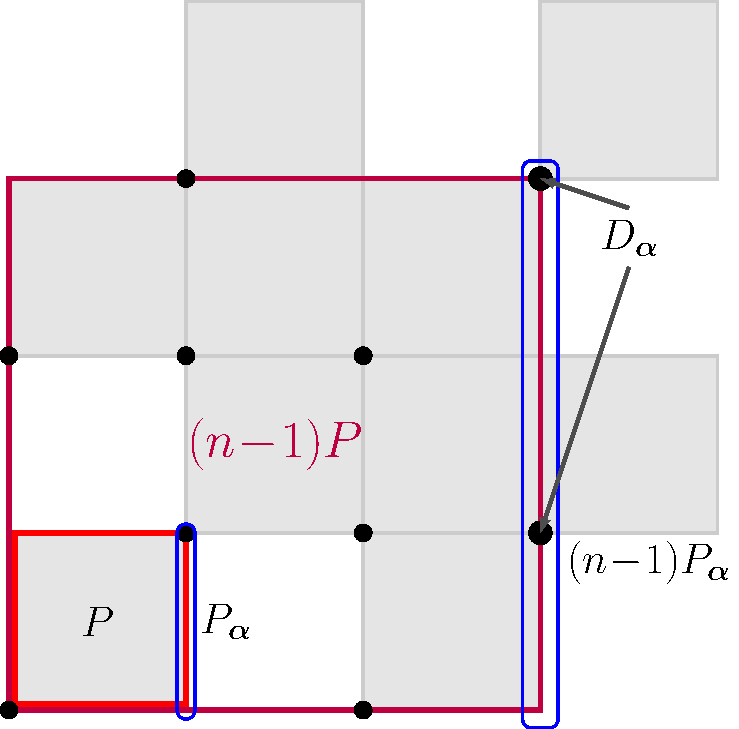
\includegraphics[width=0.45\textwidth]{faces_k.pdf}
 \caption{Множества $P_\bma$ и $D_\bma.$}
 \label{fig:faces}
\end{figure}

\begin{proposition}\label{prop:Ka}
Грань $K_\bma$ фрактального квадрата $K$ удовлетворяет уравнению $n K_\bma=K_\bma+D_\bma$, где $D_\bma=D\cap(n-1)P_\bma$.
\end{proposition}

\begin{proof}
Заметим, что $n(K\cap P_\bma)=(K+D)\cap nP_\bma.$ 
Для любого $d_i\in D$ множество $(d_i+K)\cap nP_\bma$ пусто, только если $d_i\in(n-1)P_\bma.$ 
Поэтому $d_i\in D\cap (n-1)P_\bma$. 
При этом $(d_i+K)\cap nP_\bma=d_i+K_\bma$, а потому $n K_\bma={K_\bma+D_\bma}$.
\end{proof}

Если мы спроецируем грань $K_\bma$ на координатную ось, ортогональную $\bma$, то получим {\em фрактальный отрезок} с множеством единиц $pr_\bma D_\bma$.


\begin{proposition}\label{fbma}
Пусть $K$ --- фрактальный квадрат.
\begin{itemize}[nolistsep]
\item[1.] Для любого $\bma\in A$ верно равенство $K\cap(K+\bma)=F_\bma=F_{-\bma}+\bma $;
\item[2.] Если $\bi,\bj \in I^k$, $\bi\neq \bj$ и $K_\bi\cap K_\bj\neq\0$, то $d_\bi-d_\bj=\bma$ для некоторого $\bma\in A$, и при этом 
$$K_\bi\cap K_\bj=\dfrac{d_\bi+F_\bma}{n^k}.$$
\end{itemize}
\end{proposition}

\begin{proof}
1. Поскольку $P\cap (P+\bma)=P_\bma=P_{-\bma}+\bma$, то мы имеем цепочку равенств 
$$K\cap(K+\bma)= K_\bma\cap (K_{-\bma}+\bma)=F_\bma=F_{-\bma}+\bma.$$

2. Заметим, что $S_\bi^{-1}(K_\bi\cap K_\bj)=K\cap S_\bi^{-1}(K_\bj)=K\cap (K+d_\bj-d_\bi)$. 
Поскольку по Определению \ref{refin} верно $d_\bj-d_\bi\in\zz^k$, то последние два квадрата смежны только в том случае, если $d_\bj-d_\bi$ равно некоторому $\bma\in A$. 
В этом случае $K\cap(K+d_\bj-d_\bi)=F_\bma$.
Значит $K_\bi\cap K_\bj= S_\bi(F_\bma)= \dfrac{d_\bi+F_\bma}{n^k}$. 
\end{proof}

Из Предложения \ref{fbma} следует, что для любого фрактального квадрата существует только $4$ способа пересечения смежных копий одинакового размера. 
Любое из этих пересечений является образом множества $F_{10}, F_{01}, F_{11}$ или $ F_{-1,1}$ относительно некоторого отображения $S_\bi$. 
Множества $F_{11}$ и $ F_{-1,1}$ соответствуют пересечениям противоположных углов, а потому являются одноточечными или пустыми. 

Для любых $i,j\in\{-1,1\}$ множество $F_{ij}$ является точкой $\{(i,j)\}$ если $(n-1)\cdot\left(\frac{i+1}{2},\frac{j+1}{2}\right)\in D_1$ и $(n-1)\cdot\left(\frac{-i+1}{2},\frac{-j+1}{2}\right)\in D_2$, в противном случае оно пусто. 

Множества $F_{10}, F_{01}$ соответствуют вертикальной и горизонтальной смежности копий. 
Эти множества являются пересечением противоположных сторон фрактального квадрата $K$, которые представляют из себя фрактальные отрезки.

Уравнения для множеств $F_\bma$ получаются из следующей теоремы.

\begin{theorem}\label{thm:falpha}
Для $\bma\in A\mmm\{0\}$ множество $F_\bma$ удовлетворяет уравнению
\begin{equation}\label{sideint}
 F_\bma=\bigcup\limits_{\bmb\sqsupseteq\bma} \dfrac{F_\bmb+G_{\bma\bmb}}{n}
 \end{equation}
где 
$G_{\bma\bmb}=D_\bma\cap(D_{-\bma}+n\bma-\bmb)$.
\end{theorem}

\begin{proof}
По Определению \ref{def-falpha},
\begin{equation}\label{line}
 nF_\bma=nK_\bma \cap (nK_{-\bma}+n\bma)= 
 \bigcup\limits_{d_1,d_2\in D}(K+d_1)\cap (K+d_2+n\bma).
 \end{equation}
Из $(K+d_1)\cap (K+d_2+n\bma)\neq\0$ следует, что $d_2-d_1+n\bma=\bmb$ для некоторого $\bmb\in A$.

Беря $i$-ю координату для всех записей последнего равенства, мы получаем, что
$$d_{2i}-d_{1i}+n\al_i=\be_i.$$ 
Из соотношений $\al_i,\be_i\in\{-1,0,1\}$ и $|d_{2i}-d_{1i}|\le n-1$ следует, что:\\ 
\begin{itemize}[nolistsep]
 \item[1.] если $\al_i=1$, то $\be_i>0$, а значит $\be_i=\al_i$ и $d_{2i}-d_{1i}=n-1$;
 \item[2.] если $\al_i=-1$ , то $\be_i<0$, поэтому $\be_i=\al_i$ и $d_{2i}-d_{1i}=1-n$;
 \item[3.] если $\al_i=0$ то $d_{2i}-d_{1i}=\be_i$, которое может быть $-1$, $0$ или $+1$.
\end{itemize}

По Определению \ref{Aorder}, при $\bmb\sqsupseteq\bma$ существует три возможных варианта $\bmb$ если $0\in\{\al_1,\al_2\}$.\\
С другой стороны, равенство $d_1=d_2+n\bma-\bmb$ показывает, что $d_1$ принадлежит множеству $D\cap(D+n\bma-\bmb)$, которое мы обозначим через $G_{\bma\bmb}$.\\
Для каждого $d_1\in G_{\bma\bmb}$ верно $(K+d_1)\cap (K+d_2+n\bma)= (K\cap(K+\bmb))+d_1= F_\bmb+d_1$.
Последнее равенство показывает, что $nF_\bma= \bigcup\limits_{\bmb\sqsupseteq\bma} {F_\bmb+G_{\bma\bmb}}$.
\end{proof}


\subsection{Мощность пересечений копий фрактального квадрата}

Рассмотрим фрактальный квадрат $K=\dfrac{K+D}{n}$ и пару таких копий $\dfrac{K+d_1}{n}$ и $\dfrac{K+d_2}{n}$, что $d_2=d_1+\bma$, где $\bma\in A\mmm\{0\}$.
Назовём такую пару копий {\em копиями с $\bma$-сосдедством}.
Тогда $\dfrac{K+d_1}{n}\cap\dfrac{K+d_2}{n}=\dfrac{d_1+F_\bma}{n}$, значит мощность пересечения копий $\bma$-сосдедством совпадает с мощностью множества $F_\bma$.
Уравнение множества $F_\bma$ в Теореме \ref{thm:falpha} позволяет нам оценить его мощность.

\begin{theorem}\label{fin_int}
Пусть $K=\dfrac{K+D}{n}$ --- фрактальные квадрат. Рассмотрим $F_\bma, \bma\in A\mmm\{0\}$.
\begin{itemize}[nolistsep]
 \item[(i)] Если $\#G_{\bma\bma}> 1$, то множество $F_\bma$ несчётно.
 \item[(ii)] Если $\#G_{\bma\bma}=1$, существует непустое $F_\bmb$ при $\bmb\sqsupset\bma$ и $\#G_{\bma\bmb}\geq1$, то $F_\bma$ бесконечное счётное.
 \item[(iii)] Множество $F_\bma$ конечно в следующих случаях:
 \begin{itemize}[nolistsep]
 \item[\textbf{(a)}] $\#G_{\bma\bma}=1$ и $\#F_\bmb\cdot\#G_{\bma\bmb}=0$ для каждого $\bmb\sqsupset\bma$;
 \item[\textbf{(b)}] $\#G_{\bma\bma}=0$ и существует $\bmb\sqsupset\bma$ такое, что $\#F_\bmb\cdot\#G_{\bma\bmb}\geq1$.
 \end{itemize}
\end{itemize} 
\end{theorem}

\begin{proof}
Для $\bma\in A\mmm\{0\}$ множество $F_\bma$ удовлетворяет уравнению
$F_\bma=\bigcup\limits_{\bmb\sqsupseteq\bma} \dfrac{F_\bmb+G_{\bma\bmb}}{n}$, 
где $G_{\bma\bmb}=D_\bma\cap(D_{-\bma}+n\bma-\bmb)$.
Для $\bma\in\{(1,0), (-1,0), (0,1), (0,-1)\}$ верно $\#\{\bmb:\bmb\sqsupset\bma\}=2$, при этом $\bmb\in\{(1,1), (-1,1), (1,-1), (-1,-1)\}$.
Если $\bma\in\{(1,1), (-1,1), (1,-1), (-1,-1)\}$, то $\#\{\bmb:\bmb\sqsupset\bma\}=0$.\\

Теперь, если $\bma\in\{(1,1), (-1,1), (1,-1), (-1,-1)\}$, то $\#G_{\bma\bmb}\leq1$, значит, согласно \ref{sideint}, множество $F_\bma$ не более чем одноточечно.\\

Далее предполагаем, что $\bma\in\{(1,0), (-1,0), (0,1), (0,-1)\}$.\\

(i) Если $\#G_{\bma\bma}> 1$, то $F_\bma$ содержит в себе фрактальный квадрат $Q_\bma=\dfrac{Q_\bma+G_{\bma\bma}}{n}$ с мощностью континуум.\\

(ii) Рассмтрим случай, когда $\#G_{\bma\bma}=1$, существует непустое $F_\bmb$ при $\bmb\sqsupset\bma$ и $\#G_{\bma\bmb}\geq1$. 
Такое непустое $F_\bmb$ единственное, ведь иначе $\#G_{\bma\bma}>1$.
Множество $\dfrac{F_\bmb+G_{\bma\bmb}}{n}$ конечно, поэтому $F_\bma=\bigcup\limits_{n=1}^\8 S_\bma^n$.\\

(iii {\bf a}) Пусть $G_{\bma\bma}=d_i$ и $\#F_\bmb\cdot\#G_{\bma\bmb}\geq1$ для $\bmb\sqsupset\bma$.
В этом случае $F_\bma=\dfrac{F_\bma+d_i}{n}=\dfrac{d_i}{n-1}$, то есть $F_\bma$ одноточечно.\\

(iii {\bf b}) Наконец, рассмотрим случай, когда $G_{\bma\bma}=\0$ и существует $\bmb\sqsupset\bma$ такое, что $\#F_\bmb\cdot\#G_{\bma\bmb}\geq1$.
При $G_{\bma\bma}=\0$ может существовать не более одного $\bmb\sqsupset\bma$ такого, что $F_\bmb\neq\0$, ведь иначе $G_{\bma\bma}\geq2$.
Поскольку $\#F_\bmb=1$, то $F_\bma=\dfrac{F_\bmb+G_{\bma\bmb}}{n}$ конечно, а говоря точнее, $\#F_\bma=\#G_{\bma\bmb}$.
\end{proof}

\begin{corollary}\label{onepoint} 
Если $F_\bma$ конечно, то  $\#F_\bma=\#G_{\bma\bmb}\leq\left\lfloor\dfrac{n-2}{2}\right\rfloor$.
\hfill\qed
\end{corollary}

Далее будет доказано, что фрактальный квадрат, являющийся дендритом, обладает свойством одноточечного пересечения.
Поэтому выделим случаи, при которых $F_\bma$ одноточечно:

\begin{corollary}\label{onepoint} 
Множество $F_\bma$ одноточечно, если \\
\textbf{(a)} $\#G_{\bma\bma}=1$ и $\#F_\bmb\cdot\#G_{\bma\bmb}=0$ для каждого $\bmb\sqsupset\bma$; или\\
\textbf{(b)} $\#G_{\bma\bma}=0$ и существует $\bmb\sqsupset\bma$ такое, что $\#F_\bmb\cdot\#G_{\bma\bmb}=1$.
\hfill\qed
\end{corollary}

%Рассуждения, аналогичные Теореме \ref{thm:falpha}, дают нам формулу пересечения фрактальных отрезков:
%
%\begin{proposition}
%Пусть $K_1=\dfrac{K_1+D_1}{n}$ и $K_2=\dfrac{K_2+D_2}{n}$ --- фрактальные отрезки. 
%Множество $F_0 =K_{1}\cap K_{2}$ удовлетворяет уравнению 
%\begin{equation*}
%F_0=\dfrac{F_0+G_{0}}{n}\cup\dfrac{F_{-1}+G_{-1}}{n}\cup\dfrac{F_{1}+G_{1}}{n}, 
%\end{equation*}
%где для любого $a\in\{-1,0,1\}$ верно, что $G_{a}=D_1\cap(D_2-a)$ и $F_a=K_1\cap (K_2+a)$.\\
%Если $F_{1}\neq\0$, то $0\in D_2$,$(n-1)\in D_1$ и $F_1=\{1\}$.\\ 
%Если же $F_{-1}\neq\0$, то $0\in D_1$, $(n-1)\in D_2$ и $F_{-1}=\{0\}$. \hfill\qed
%\end{proposition}
%
%Пусть $K_1$ and $K_2$ -- фрактальные отрезки порядка $n$ с множествами единиц $D_1$ и $D_2$ такими, что $0\in D_1$ и $n-1\in D_2$, а следовательно $0\in K_1$ и $1\in K_2$.
%Если $k\in D_1$ и $k-1\in D_2$, то $k/n\in K_1\cap K_2$ и такую точку будем называть {\em точкой пересечения} $K_1$ и $K_2$.
%
%\begin{corollary}\label{fin_int}
%Пусть $K_1=\dfrac{K_1+D_1}{n}$ и $K_2=\dfrac{K_2+D_2}{n}$ --- фрактальные отрезки.
%\begin{itemize}[nolistsep]
% \item[(i)] Если $\#G_0> 1$, то мнжество $F_0$ несчётно.
% \item[(ii)] Если $\#G_0\le 1$, то только одно из множеств $F_{-1},F_1$ непусто и $F_0$ счётно.
% \item[(iii)] Множество $F_0$ конечно в следующих случаях:
% \begin{itemize}[nolistsep]
% \item[\textbf{(a)}] $\#G_0=1$ и $(F_{-1}+G_{-1})\cup(F_{1}+G_{1})=\0$;
% \item[\textbf{(b)}] $\#G_0=0$ и $(F_{-1}+G_{-1})\cup(F_{1}+G_{1})\neq\0$.
% \end{itemize}
%\end{itemize} 
%\end{corollary}
%
%\begin{proof}
%Поскольку при $i\in\{-1,+1\}$ верно $\#F_{i}\le 1$, то множества $\dfrac{F_{i}+G_{i}}{n}$ конечны.
%
%(i) Заметим, что ели $\#G_0>1$, то $F_0$ содержит множество $Q_0=\dfrac{Q_0+G_0}{n}$, являющееся несчётным.\\
%
%(ii) Предположим, что $\#G_0=1$, т.е. $G_0=\{d_0\}$, и $(F_1+G_1)\cup(F_{-1}+G_{-1})\neq\0$. \vspace{1mm}\\
%Пусть $\widetilde{d}_0:=\dfrac{d_0}{n-1}$ --- неподвижная точка гомотетии $S_{d_0}(x)=\dfrac{x+d_0}{n}$.
%Для любого $x_0\in\dfrac{(F_1+G_{1})\cup(F_{-1}+G_{-1})}{n} $ множество $F_0$ содержит последовательность $x_k=\dfrac{x_0-\widetilde{d}_0}{n^k}+\widetilde{d}_0$.
%Поэтому $F_0$ --- бесконечное счётное множество.\\
%
%(iii) В случае \textbf{(a)} получаем $F_0=\{\widetilde{d}_0\},$ поэтому $\#F_0=1$.\\
%
%В случае \textbf{(b)} получаем $n F_0=(F_1+G_1)\cup (F_{-1}+G_{-1})$, поэтому $\#F_0=\#F_{1}\cdot\#G_1+\#F_{-1}\cdot\#G_{-1}<\8$.
%\end{proof}
%
%\begin{corollary}\label{onepoint} 
%Множество $F_0$ одноточечно, если \\
%\textbf{(a)} $\#G_0=1$ и $\#F_{1}\cdot\#G_1+\#F_{-1}\cdot\#G_{-1}=0$; или\\
%\textbf{(b)} $G_0=\0$ и 
%$\#F_{1}\cdot\#G_1+\#F_{-1}\cdot\#G_{-1}=1$. 
%\hfill\qed
%\end{corollary}



% \begin{corollary}
% If a fractal square $K$ of order $n$ possesses
% finite intersection property, then for any nonequal two pieces $K_\bi,K_\bj$ of the same rank, $$\#K_\bi\cap K_\bj\leq \left\lfloor\frac{n-2}{2}\right\rfloor$$
% \end{corollary}


% \begin{figure}[H]
% \centering
% \includegraphics[width=\textwidth]{2fip.pdf}
% \caption{A fractal square of order 6 possessing 2 point intersection property. The points of self-similar boundary are indicated by arrows. Blue and red arrows show the junction ponts.}
% \label{fig:2fip}
%\end{figure}

\section{Самоподобная граница и главное дерево фрактального квадрата}

\begin{proposition}
\label{thm:den_necessary_sufficient}
Если фрактальный квадрат $K$ является дендритом, то он обладает свойством одноточечного пересечения.
\end{proposition}

\begin{proof}
Пересечение $K_\bi\cap K_\bj$ двух копий фрактального квадрата, являющегося дендритом, будет связно, следовательно оно будет либо точкой, либо отрезком.
Последнее возможно, когда пересечение $K_\bi\cap K_\bj$ есть полная сторона, поскольку фрактальный отрезок $L$ содержит отрезок тогда и только тогда, когда $L=[0, 1]$. 

Предположим, что $K$ --- связный фрактальный квадрат с пересечением своих копий по полной стороне. 
Тогда, с точностью до вращения, $K$ содержит $[0,1]\times\{0,1\}$.
Такой пример показан на Рисунке \ref{fig:line_int}.

В этом случае множество $D$ содержит подмножество $ \{0,\ldots,n-1\}\times \{0,n-1\}$, значит $K$ содержит подмножество $L=[0,1]\times\{0,1/n\}$. 
Для каждого из множеств $K_{0k}=\dfrac{K+(0,k)}{n}$, пересечение $K_{0k}\cap L$ есть пара параллельных отрезков. 
По связности $K_{0k}$ существует путь $\ga_{0k}\IN K_{0k}$ соединяющий эти  отрезки. 

Объединение $L\cup\ga_{00}\cap\ga_{n-1,0}$ содержит замкнутую дугу, значит $K$ не является дендритом. 
\end{proof}

\begin{figure}[H]
 \centering
 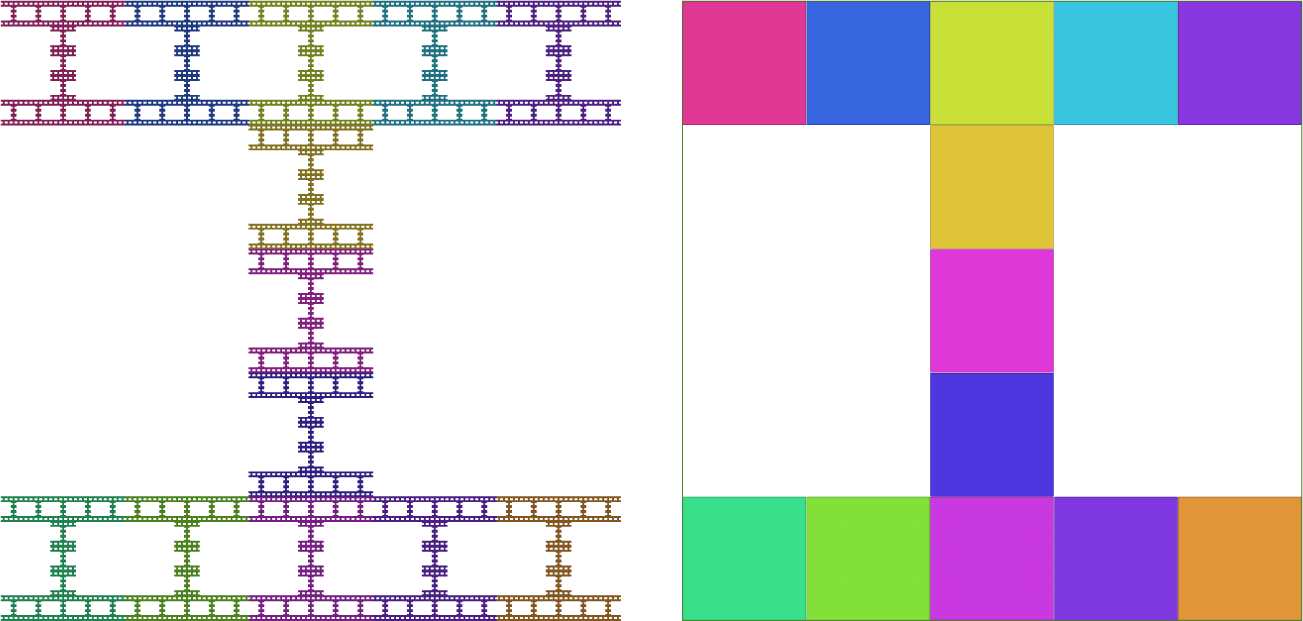
\includegraphics[width=0.8\textwidth]{line_int.png}
 \caption{Фрактальный квадрат с пересечением по полной стороне.}
 \label{fig:line_int}
\end{figure}

\begin{corollary}
Фрактальный квадрат $K$ является дендритом тогда и только тогда, когда его двудольный граф пересечений является деревом.\hfill\qed
\end{corollary}

Рассмотрим множество $A=\{-1,0,1\}^2$ и соответствующее ему множество граней квадрата. 
Для фрактального квадрата $K$ с множеством единиц $D$ мы определим множество 
$$A_D=\{\bma\in A\mmm\{(0,0)\}: D\cap(D+\bma)\neq\0\}.$$ 
Множество $A_D$ --- это множество тех $\bma\in A$ для которых существуют копии $K_i, K_j$ такие, что $d_j-d_i=\bma$ и, следовательно, имеющие общие граничные точки. 
Для таких копий их общая граница равна $S_i(F_\bma)=S_j(F_{-\bma})$. 

Следующее утверждение очевидно:\\

\begin{proposition}
Самоподобная граница $\dd K$ фрактального квадрата $K$ есть объединение
\begin{equation}
 \dd K=\bigcup\limits_{\bma\in A_D}F_\bma.
\end{equation}
\end{proposition}

Заметим, что для любой копии $K_\bi$ из $K$ топологическая граница $K_\bi$ в $K$ является подмножеством в 
$S_\bi(\dd K)$. 
Таким образом если путь $\ga\IN K$ имеет концы $a\in K_\bi$ и $b\in K\mmm K_\bi$, то $\ga$ содержит $S_\bi(\dd K)$.

\begin{theorem}\label{ssboundary}
Пусть $K$ --- фрактальный квадрат, являющийся дендритом и не являющийся интервалом. 
Существуют следующие типы самоподобных границ $\dd K$:\\
Если $\dd K=F_\bma\cup F_{-\bma}\cup F_\bmb\cup F_{-\bmb}$ то $\dd K$ будет иметь:\\
тип {\bf A} если $\bma=(1,0)$, $ \bmb=(0,1)$;\\ 
тип {\bf B} если $\bma=(1,1)$, $ \bmb=(1,-1)$; \\
тип {\bf C} если $\bma=(1,1) \text{ или } (1,-1),\bmb=(1,0) \text{ или }(0,1)$.\\
Для типа {\bf D} будет верно $\dd K=F_{(1,0)}\cup F_{(-1,0)}\cup F_{(0,1)}\cup F_{(0,-1)}\cup F_\bmb\cup F_{-\bmb}$,\\ где
 $\bmb=(\be_1,\be_2)=(1,1) \mbox{ or }(1,-1)$.
 
Для типов {\bf A, B, C} множество $\dd K$ состоит из $4$ точек. 
Тип {\bf D} может иметь границу $\dd K$ из $6$ точек (будем называть такой случай как тип {\bf D6}) или, в вырожденном случае, из $3$ точек (будем называть такой случай как тип {\bf D3}).
\end{theorem}

\noindent Вырожденный случай {\bf D3} возникает, если существуют $\bma\in\{(1,0),(-1,0)\}$ и $\bmb\in\{(0,1),(0,-1)\}$ такие, что $F_\bma=F_\bmb$.

\begin{figure}[H]
\centering
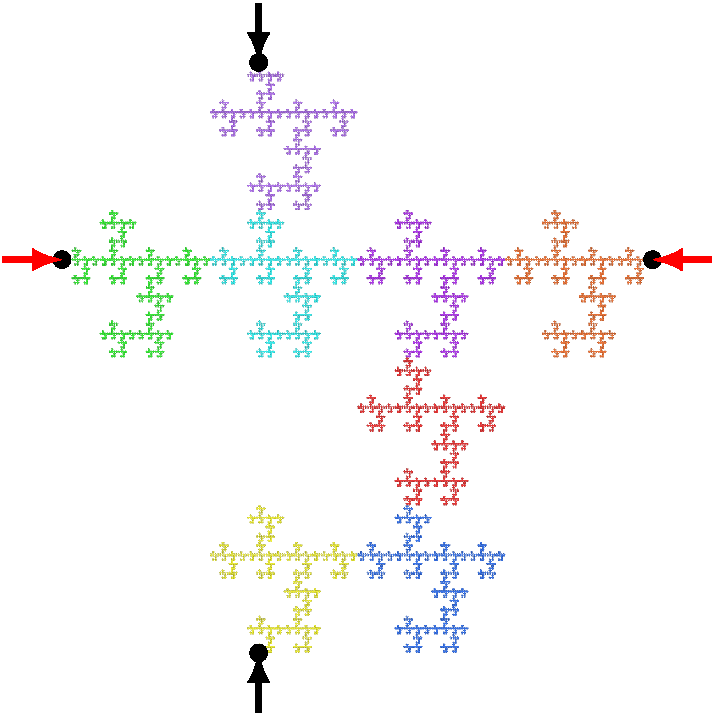
\includegraphics[width=0.3\textwidth]{A_type.pdf}
\hfill
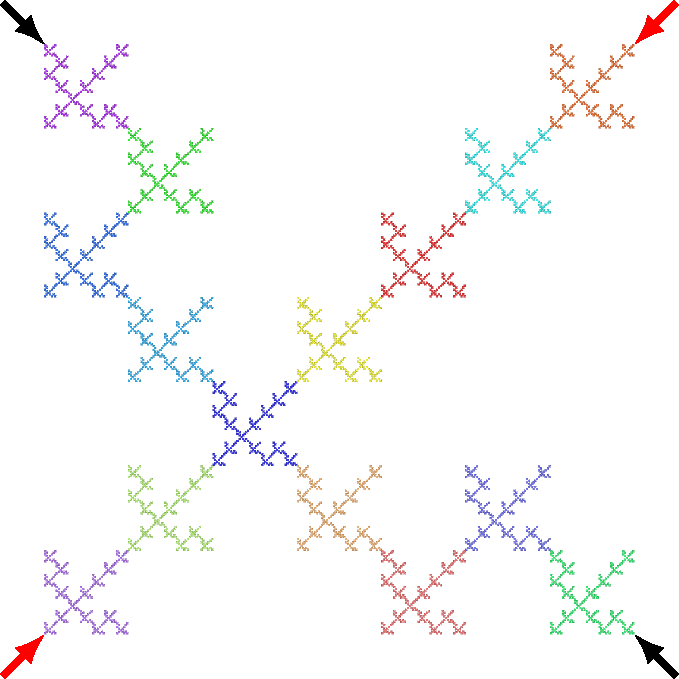
\includegraphics[width=0.3\textwidth]{B_type.pdf}
\hfill
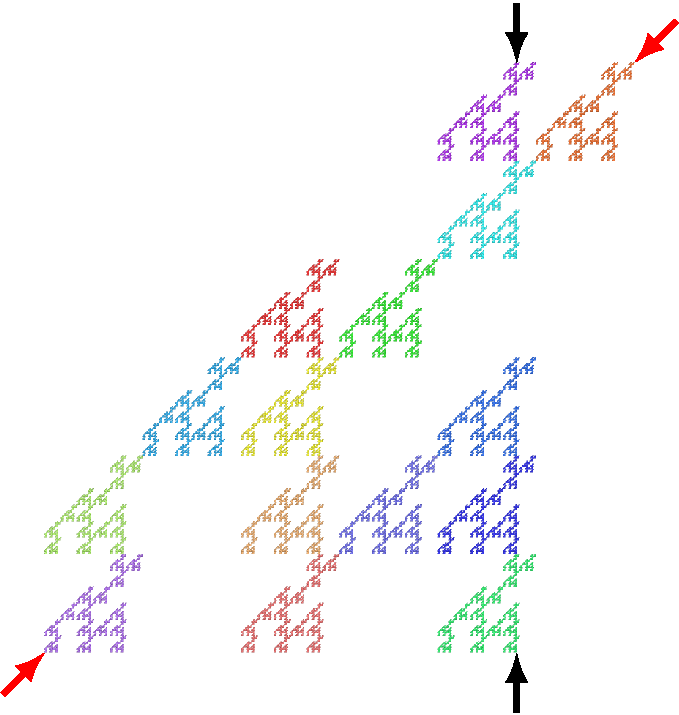
\includegraphics[width=0.3\textwidth]{C_type.pdf}\\
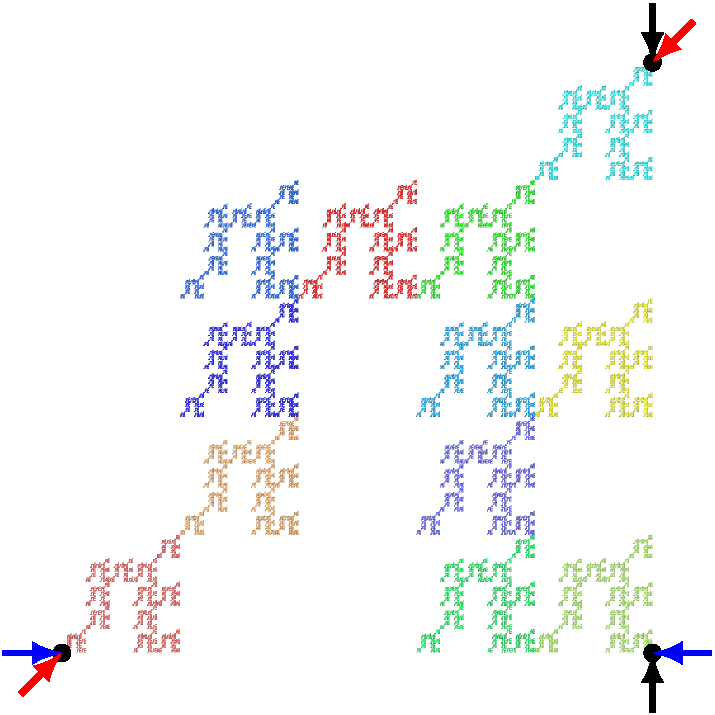
\includegraphics[width=0.3\textwidth]{D3_type.pdf}
\hfill
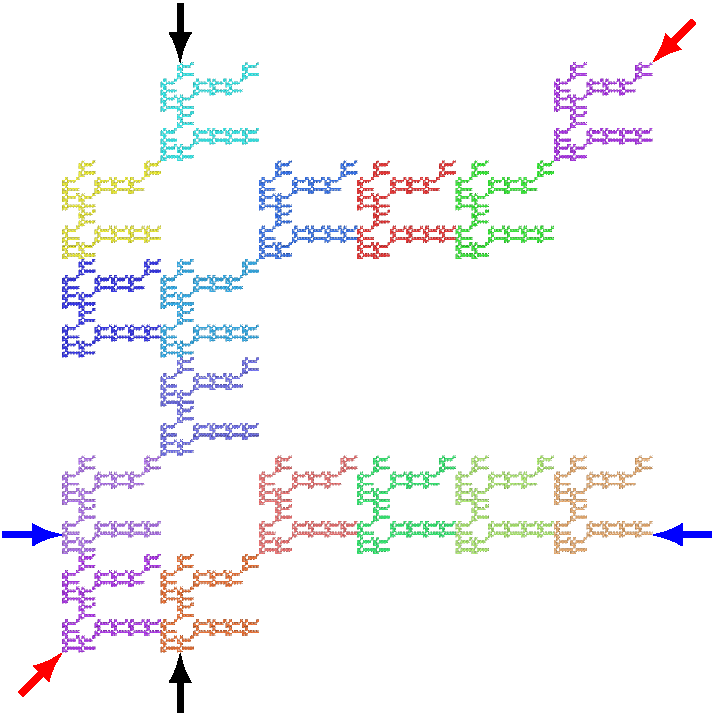
\includegraphics[width=0.3\textwidth]{D6_type.pdf}
\caption{Фрактальные квадраты типа {\bf A}, {\bf B}, {\bf C}, {\bf D3} и {\bf D6}. Стрелками одного цвета показана пара противоположных точек самоподобной границы, которые лежат в множествах $F_\bma$ и $F_{-\bma}$. В типе {\bf D3} каждая точка самоподобной границе принадлежит сразу двум множествам из системы $\{F_\bma\ :\ \bma\in A\mmm\{0\}\}$.}
\end{figure}

\begin{proof}
Если для некоторого $\bma\in A$ самоподобная граница $\dd K=F_\bma\cup F_{-\bma}$, то $K$  есть интервал с концами $F_\bma$ и $ F_{-\bma}$.
 
Если множество $A_D$ содержит $(1,1),(1,-1)$ и $\bma=(0,1)$ или $\bma=(1,0)$, то $\#G_\bma\geq 2$, а значит, согласно Следствию \ref{fin_int}, $F_\bma$ несчётно, что является невозможным, если $K$  является дендритом, следовательно $\bma\notin A_D$. 
Все остальные случаи перечисляются в типах {\bf A, B, C, D}.

Для типа {\bf A} множество $\dd K$ может состоять только из четырёх точек. 
Если хоть одна из этих точек является угловой (углом квадрата), то $\dd K$ содержит ровно две угловых точки, которые являются концами на некоторой стороне квадрата $P$ и три точки из $\dd K$ лежат на этой грани.

Предположим, что $\dd K$ содержит $3$ угловые точки, например $(1,0),(0,0)$ и $(0,1)$.
Отсюда следует, что $F_{(1,-1)}\neq\0$.
Если это так, то множество $\dfrac{D+P}{n}$ связно и содержит точки $(1,0)$ и $(0,1)$. 
Мы утверждаем, что в этом случае $G_{(-1,1)}=(D\cap (D+(1,-1))\neq\0$.
 
Действительно, пусть $D'$ --- подмножество в $D$ удовлетворяющее условиям:\\
1. Множество $D'+P$ связно;\\
2. $D'\cap (D'+(1,-1))=\varnothing$;\\
3. $(0,n-1)\in D'$. 

Тогда $D'$ равно либо $\{0\}\times\{k,\ldots,n-1\}$, либо $\{k,\ldots,n-1\}\times\{n-1\}$ для некоторого $0\leq k\leq n-1$.
Это наблюдение доказывает наше утверждение.
 
Итак, $F_{(1,-1)}\neq\0$, $(1,-1)\in A_D$ означает, что мы столкнулись с типом {\bf D}. 
 
Аналогичные рассуждения показывают, что в типе {\bf C} множество $\dd K$ может состоять только из четырёх точек. 
Тип {\bf B} очевиден.

Для типа {\bf D} граница $\dd K=F_{(1,0)}\cup F_{(-1,0)}\cup F_{(0,1)}\cup F_{(0,-1)}\cup F_{(1,1)}\cup F_{(-1,-1)}$.
Пусть $\bma\in\{(1,0),(-1,0)\}$ и $\bmb\in\{(0,1),(0,-1)\}$. 
Тогда равенства $F_\bma=F_{-\bmb}$, $F_{\bmb}=F_{\bma+\bmb}$ и $F_{-\bma}=F_{-\bma-\bmb}$ эквивалентны и $\dd K=F_{-\bma}\cup F_\bma\cup F_\bmb$. 

Это показывает что для типа {\bf D} из $\#\dd K<6$ следует $\#\dd K=3$. 
Обозначим получившиеся два подтипа как {\bf D3} и {\bf D6}.
\end{proof}

Как следует из Теоремы \ref{ssboundary}, самоподобная граница фрактального квадрата, являющегося дендритом, состоит из $3$, $4$ или $6$ точек.


% \begin{definition}\label{def:mtree}
% Let $K$ be a FSD possessing finite self-similar boundary $\dd K$. 
% The minimal subdendrite $\hat\ga\IN K$, containing $\dd K$ is called the {\em main tree} of the dendrite $K$.
% \end{definition}

% We provide some statements concerning the main tree $\hat\ga$ of a self-similar dendrite $K$ with a finite self-similar boundary; see \cite{polden}.\\
% 1. If $x\in \hat\ga$ and for any component $Q$ of $K\mmm\{x\}$, $Q\cap\dd K\neq\0$, then $Ord(x,K)=Ord(x,\hat\ga)$.\\
% 2. If $x$ is a cut point of dendrite $K$, then either $x\in S_\bi(\dd K)$ for some $\bi$, or for any component $Q$ of $K\mmm\{x\}$, $Q\cap\dd K\neq\0$.\\
% 3. The set $CP(K)$ of cut points of $K$ is the union of all sets $S_\bi(\hat\ga), \bi\in I^*$. 
% Therefore, $\dim_H(CP(K))=\dim_H(\hat\ga)$.


\section{Порядок точек ветвления фрактального квадрата, являющегося дендритом}

\subsection{Запретные комбинации в множествах единиц для разных типов фрактальных квадратов, являющихся дендритами}

Для фрактального квадрата, являющегося дендритом, в множестве единиц существуют комбинации единиц, которые не могут встречаться в $D^k$ для любого $k$. 
В следующей лемме рассматриваются такие комбинации. 
мы говорим, что множество $Q\IN \zz^2$ {\em  запретное} (для данного типа фрактального квадрата $K$), если для любых $k\in\nn$ и $\widetilde d\in D^k$ верно
$\widetilde d+Q\not\IN D^k.$

\begin{lemma}\label{quadruples}
Следующие комбинации единиц $Q$ запретные:
\begin{itemize}[nolistsep]
\item[a)] $\{(0,0), (1,0)\} $ и $\{(0,0), (0,1)\} $ для типа {\bf B} ;
\item[b)] $\{(0,0), (0,1), (1,0), (1,1)\}$ для всех типов, кроме {\bf C};
\item[c)] $\{(0,0),\bma,\bmb,\bma+\bmb\}$ для типа {\bf C};
\item[d3)] тройка $\{a_1, a_2, a_3\}$ для типа {\bf D3}, если $\dd K=\{a_1,a_2, a_3\}$;
\item[d6)] тройки $\{(0,0),(\be_1,0),\bmb)\}$ и $\{(0,0),(0,\be_2),\bmb)\}$ для типа {\bf D6}. 
\end{itemize}
\end{lemma}

\begin{proof} 
Случай a) очевиден, так как для любого $\bma\in\{(0,1),(1,0)\}$ множество $F_\bma$ несчётно.

Чтобы доказать, что множество $Q$ целочисленных векторов {\em запретное} для других типов, мы убедимся, что множество $Q+K$ содержит непересекающиеся замкнутые контуры.

(b) для типов {\bf A, D6} предположим, что $\bma=(1,0), \bmb=(0,1)$ и $F_{-\bma}=\{(0,b)\}, F_{-\bmb}=\{(a,0)\}$, где $a,b$ принадлежит интервалу $[0,1]$.
Поскольку одно из множеств $F_{(1,1)}$ или $F_{(1,-1)}$ пусто, то существует открытый квадрат $P_1=\dfrac{x+\dot P}{n}$, $x\in \{(-1,-1),(0,-1), (-1,0), (0,0)\}$ который имеет пустое пересечение $Q+K$. 
Обозначим $x_1=(a,0)$, 
$x_2=(0,b)$, $x_3=(a-1,0)$, $x_4=(0,b-1)$. 
Пусть $\ga(x_1,x_2)$, $\ga(x_2,x_3)$,$\ga(x_3,x_4)$ и $\ga(x_4,x_1)$ --- поддуги в $K$, $-\bma+K$, $-\bma-\bmb+K$ и $-\bmb+K$ соответственно.
Они образуют дугу в $Q+K$, огибающую $P_1$, а значит эта дуга нестягиваема. 

Если для типа {\bf A} имеем $F_\bma=(0,1)$, а квадрат $P_1=\dfrac{x+\dot P}{n}$ имеет пустое пересечение $Q+K$ для обоих $x\in\{(-1,0), (0,0)\}$, то рассуждения остаются аналогичными.

\begin{figure}[H]
    \centering
    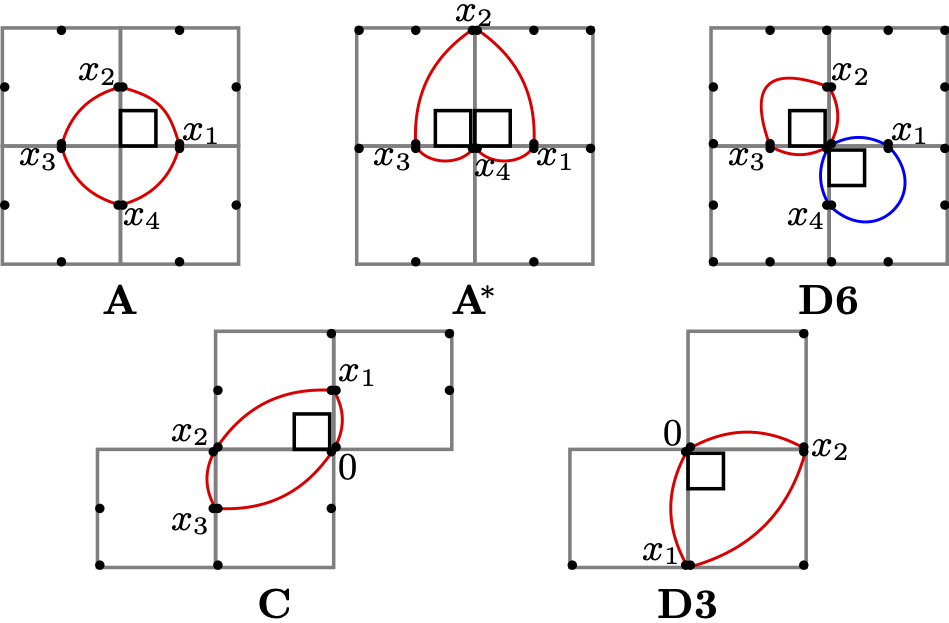
\includegraphics[width=.8\textwidth]{quadruples.png}
    \caption{Построение нестягиваемых петель в запретных комбинациях для типов {\bf A, C} и {\bf D}.}
    \label{forbid}
\end{figure}

Аналогичным образом доказываются утверждения c), d3) и d6).
Мы выбираем вершину в $Q+K$, около которой существует открытый квадрат $P_1=\dfrac{x+\dot P}{n}$, имеющий пустое пересечение с $Q+K$, и теперь формируем нестягиваемую петлю из поддуг $\ga(x_i,x_j)$, соединяющих граничные точки множеств $q_i+K$.
Выбор точек и дуг показан на Рисунке \ref{forbid}.
\end{proof}


\subsection{Количество угловых точек и их порядки ветвления}

\begin{theorem}\label{thm:vertex_branching}
Пусть $K$ --- фрактальный квадрат, являющийся дендритом.
Для любой угловой точки $a\in K$,
 $Ord(a,K)\leq 2$.
\end{theorem}

\begin{proof}\label{proof:vertex_branching}
Заметим, что для любой копии $K_\bi\ni a$ верно, что 
$K_\bi\mmm \{a\}=S_\bi(K\mmm \{a\})$. 
Следовательно, если $Q$ является компонентой в $K\mmm \{a\}$, то $Q\cap K_\bi=S_\bi(Q)$. 
Пусть $Q_1,\ldots, Q_k$ --- множество всех этих компонент, тогда $K\mmm \{a\}=\bigsqcup \limits_{j=1}^kQ_j$ и $\dd K\mmm \{a\}=\bigsqcup \limits_{j=1}^k(Q_j\cap\dd K)$, поэтому $\dd K_\bi\mmm \{a\}=\bigsqcup \limits_{j=1}^k(Q_j\cap\dd K_\bi)$. 
Число $k$ пересечений в последнем равенстве не больше чем $3$, так как эти пересечения соответствуют двум сторонам и одной вершине, противоположным точке $a$. 
Каждое из этих пересечений содержит не более одной точки, и то же самое верно для соответствующих пересечений $Q_j\cap\dd K$.

Без потери общности предположим, что  $a=(0,0)$.  
таким образом $Q_1\cap K_{10}=F_{10}$ если $d_{(1,0)}\in D$, $Q_2\cap K_{01}=F_{01}$ если $d_{(0,1)}\in D$ и $Q_3\cap K_{11}=F_{11}$ если $d_{(1,1)}\in D$.

Для типа {\bf A} имеем $F_{11}=\0$, значит $Ord(a,K)\leq 2$.
Для типа {\bf B} верно $F_{10}=F_{01}=\0$, следовательно $Ord(a,K)=1$.
И для типа {\bf C} либо $F_{10}=\0$, либо $F_{01}=\0$, следовательно $Ord(a,K)\leq 2$.

Предположим, что порядок угловой точки $a=(0,0)$ равен $3$.
Тогда единицы $(0,0)$, $(1,0)$, $(0,1)$ и $(1,1)$ содержатся $D$. 
По Лемме \ref{quadruples} это невозможно.

Это противоречие показывает, что для типа {\bf D} $Ord(a,K)\leq 2$.
\end{proof}

Теперь рассмотрим, сколько угловых точек может быть для каждого из типов: {\bf A, B, C, D}.

\begin{theorem}\label{thm:corner}
Пусть $K$ --- фрактальный квадрат, являющийся дендритом. \\
Если $K$ --- дендрит типа  {\bf A}, то у него могут быть две угловые точки с порядками $2,1$ или $1,1$, может быть одна угловая точка порядка $1$ или $2$, а также могут вовсе отсутствовать угловые точки.\\
Если $K$ --- дендрит типа  {\bf B}, то у него четыре угловые точки порядка $1$.\\
Если $K$ --- дендрит типа  {\bf C}, то у него две угловые точки, порядки которых могут быть равны $1$ или $2$.\\
Если же $K$ --- дендрит типа  {\bf D}, то он может иметь две угловые точки порядков $\le 2$ для подтипа {\bf D6} или три угловые точки порядка $1$ для подтипа {\bf D3}.
\end{theorem}

\begin{proof}
$K$ содержит $4$ угловые точки тогда и только тогда, когда он относится к типу {\bf B}. 
$K$  имеет $3$ угловые точки тогда и только тогда, когда он относится к типу {\bf D3}. 
Если $K$ имеет $2$ противоположные угловые точки, то он относится к типу {\bf C} или {\bf D6}.

Как следует из доказательства Теоремы \ref{ssboundary}, если $K$ относится к типу {\bf A}, то он не может содержать пару противоположных угловых точек. 
Значит $K$ содержит не более двух угловых точек, которые являются концами некоторой стороны квадрата $P$. 

Пусть этими двумя точками являются $(0,0)$ и $(1,0)$, тогда $\dd K=\{(0,0), (a,0), (1,0), (a,1)\}$, где $a=\dfrac{p}{n-1}$ и $p\in \{2, \ldots, n-2\}$. 
Если порядки обеих точек, $(0,0)$ и $(1,0)$,  равны $2$, то $\{(0,1), (n-1,1)\}\IN D$, поскольку каждая из копий $\dfrac{K}{n}$ и $\dfrac{n-1+K}{n}$ должна иметь двух соседей. 
В этом случае $F_{(1,0)}$ несчётно, что невозможно.
Следовательно порядки ветвления этих двух точек равны $2,1$ или $1,1$.

Случай с типом {\bf B} очевиден.
В случае с типом {\bf C} множество $\dd K$ содержит ровно $2$ противоположные угловые точки, порядки которых не превышают $2$.

Предположим, что $K$ относится к типу {\bf D3} и его угловыми точками являются $(0,0)$, $(1,0)$ и $(1,1)$. 
Если $Ord((0,0),K)=2$, то у копии с единицей $(0,0)$ есть $2$ соседа. 
Следовательно $(0,0)$, $(1,0)$ и $(1,1)$ содержатся в  $D$. 
По Лемме \ref{quadruples} эта комбинация единиц является запретной.

Эти же рассуждения можно применить, чтобы показать, что точка $(1,0)$ не может иметь порядок $2$.

Для типа {\bf D6} существуют ровно две противоположные угловые точки, лежащие в границе $\dd K$. 
%\red{Примеры показывают, что для этих двух точек возможна каждая из комбинация порядков ветвлений: и $1,1$, и $1,2$, и $2,2$.}
\end{proof} 

% The Figures \ref{fig:A_type_Three}, \ref{fig:C_type_Three} and
% \ref{fig:D6_type_Three} show the corner points of  order two for the types {\bf A, C, D6} respectively.
% \begin{figure}[H]
%     \centering
%     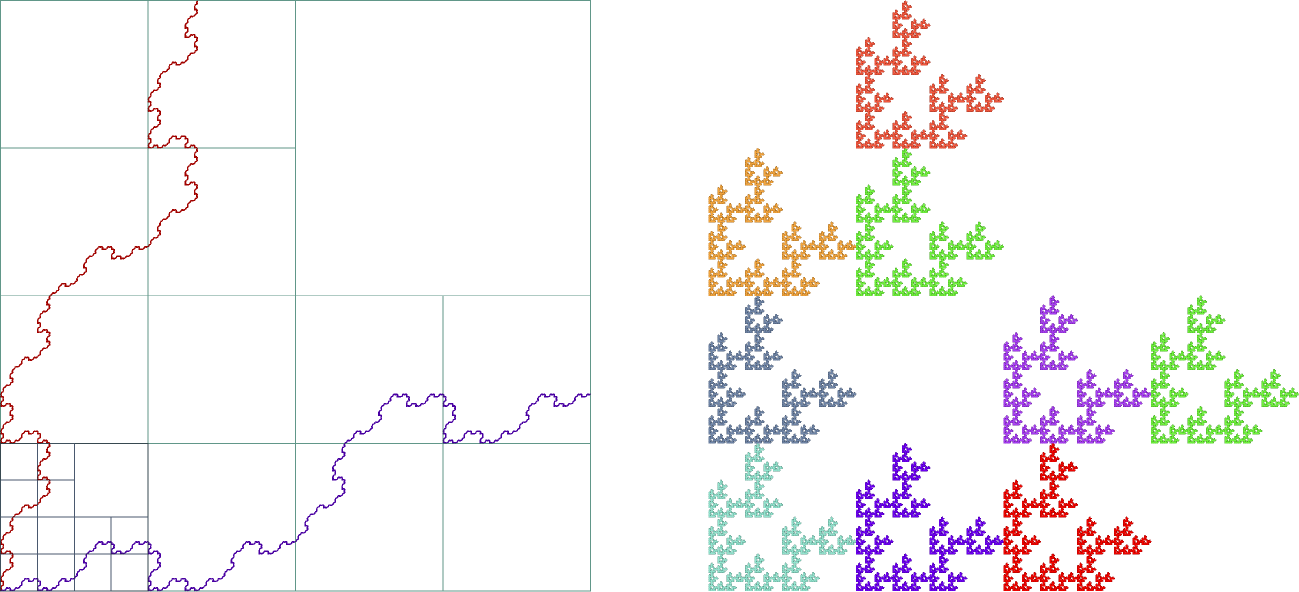
\includegraphics[width=0.7\textwidth]{A_type_Three.png}
%     \caption{}
%     \label{fig:A_type_Three}
% \end{figure}

\begin{figure}[H]
    \centering
    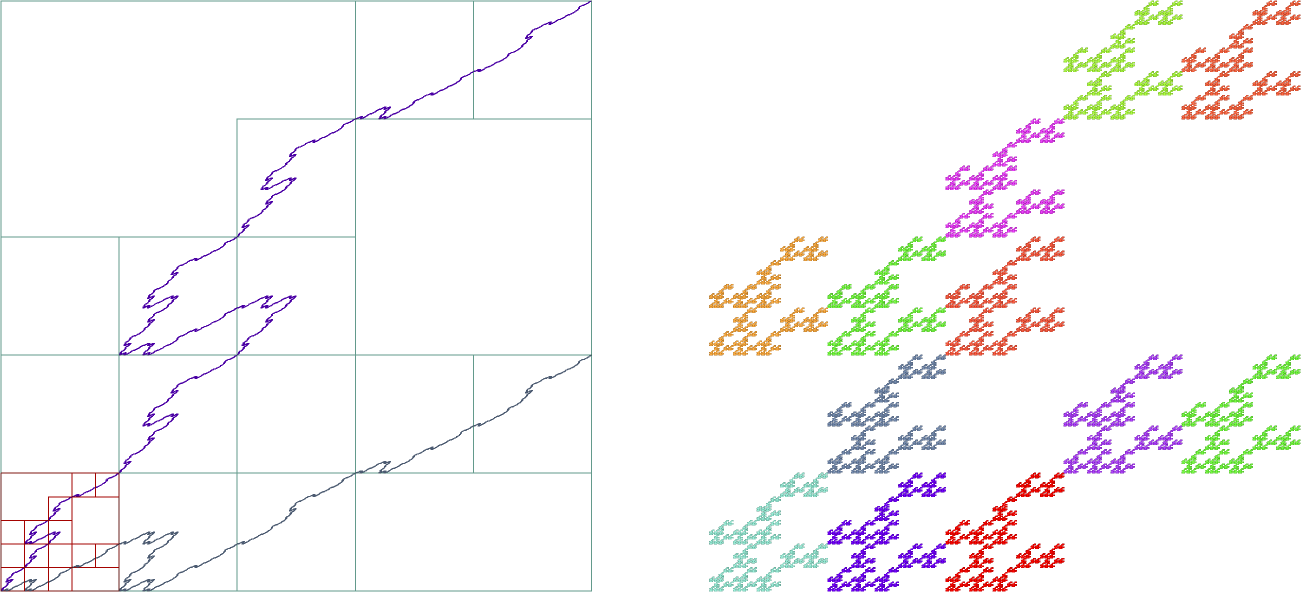
\includegraphics[width=0.7\textwidth]{C_type_Three.png}
    \caption{Угловая точка порядка 2 для типа {\bf C} и две главные дуги, содержащие ее.} 
    \label{fig:C_type_Three}
\end{figure}

% \begin{figure}[H]
%     \centering
%     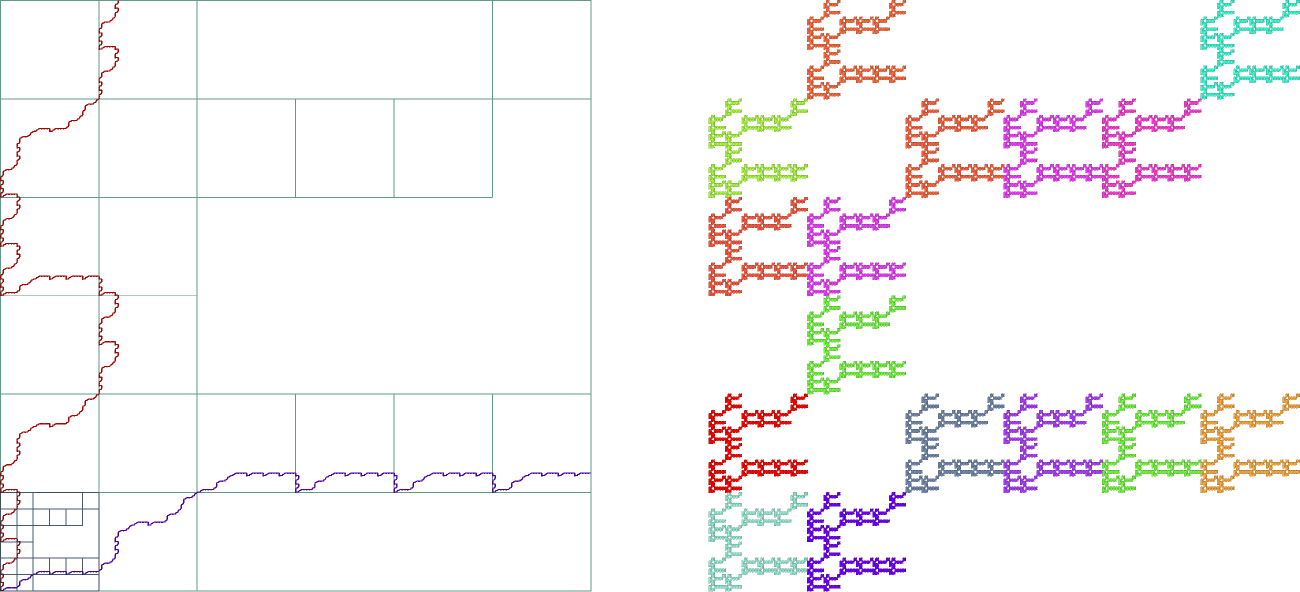
\includegraphics[width=0.7\textwidth]{D6_type_Three.png}
%     \caption{}
%     \label{fig:D6_type_Three}
% \end{figure}

\begin{theorem}\label{order}
Пусть $K$ --- фрактальный квадрат, являющийся дендритом. 
Тогда для любого  $x\in K$ верно $Ord(x,K)\le 4$.\\
Если $K$ относится к типу {\bf D} и $x\notin S_\bi(\dd K)$ для любого $\bi\in I^*$, то $Ord(x,K)\le 3$.\\
Если $K$ относится к типу {\bf D3} и $x\in \dd K_\bi$ для некоторого $\bi\in I^*$, то $Ord(x, K)\le 3$.
\end{theorem}

\begin{proof}\label{proof:point_branching}
Пусть $Ord(x,K)=l$.
Тогда существует $l$ жордановых дуг $\{\ga_i\}_{i=1}^l$ в $K$ с общим концом $x$, причем таких, что дуги $\ga_i\mmm \{x\}$ непересекаются.
Существует натуральное $p>0$ такое, что для каждого $\ga_i$ его диаметр $|\ga_i|$ больше, чем $\sqrt{2}n^{-p}$.
С учётом Леммы \ref{quadruples} можно увидеть, что существуют $1$, $2$ или $3$ мультииндекса $\bi=i_1i_2\ldots i_p$ таких, что $x\in S_\bi(K)$.

В случае (1), когда такое $\bi$ единственно, каждая дуга $\{\ga_i\}$ проходит в одну из соседних копий порядка $n^p$ для $K_\bi$ через одну из точекк $\dd K_\bi$ (см. Рисунок \ref{fig:case1}). 
Таким образом, число $l$ не превышает количества соседей для $K_\bi$  и числа точек в $\dd K_\bi$. 

Аналогично можно рассуждать в случае (2), когда $x\in K_\bi\cap K_\bj$ и $x$ лежит внутри (не в конце) общей стороны квадратов $S_\bi(P)$ и $S_\bj(P)$ (см. Рисунок \ref{fig:case2}), и в случае (3), когда $x$ является общей угловой точкой для двух или трех квадратов (см. Рисунок \ref{fig:case3}). 
В этих случаях число $l$ не больше числа соседей для тех $K_\bi$, которые содержат $x$ и соответствующие точки их границ.

\textbf{(1)}
Пусть $x\in \dot K_\bi$.
Для типов {\bf A, B, C} число $l\leq 4$.

Для типа {\bf D} верно, что $l\le 3$. 
Действительно, выбирая четвёрку из $6$ возможных соседей копии $K_\bi$, мы получаем запретную комбинацию. 
\begin{figure}[H]
    \centering
    %\includestandalone[width=1\textwidth]{tikzpictures/case1}
    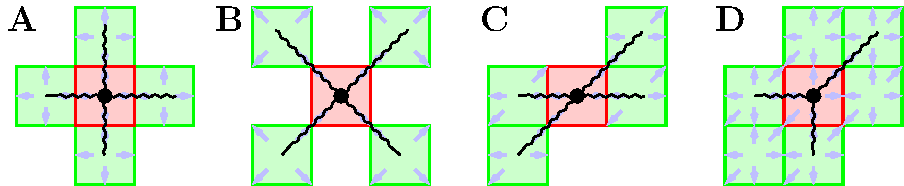
\includegraphics[width=\textwidth]{case1.pdf}
    \caption{Порядки ветвления внутренних точек в типах \textbf{A}, \textbf{B}, \textbf{C} и \textbf{D}}
    \label{fig:case1}
\end{figure}

\begin{figure}[H]
    \centering
    %\includestandalone[width=0.66\textwidth]{tikzpictures/case2}
    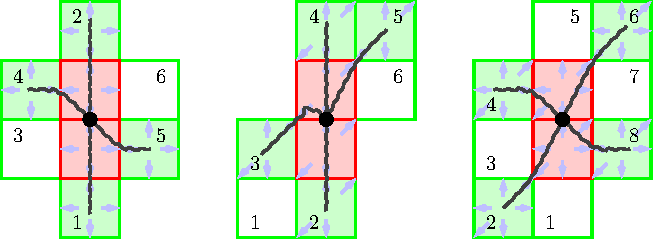
\includegraphics[width=0.73\textwidth]{case2.pdf}
    \caption{Доступные соседи точки $x$ на общей стороне для типов \textbf{A}, \textbf{C} и \textbf{D6}}. 
    \label{fig:case2}
\end{figure}


\textbf{(2)}
Пусть $x\in S_\bi(\dd K)$ --- внутренняя точка общей стороны для $S_\bi(P)$ и $S_\bj(P)$.
Это возможно только в случаях \textbf{A}, \textbf{C} и \textbf{D6}.

В этом случае число доступных соседей $S_\bi(P)\cup S_\bj(P)$ не может превышать $4$ согласно Лемме \ref{quadruples}.

\begin{figure}[H]
    \centering
%\includestandalone[width=0.7\textwidth]{tikzpictures/case3}
    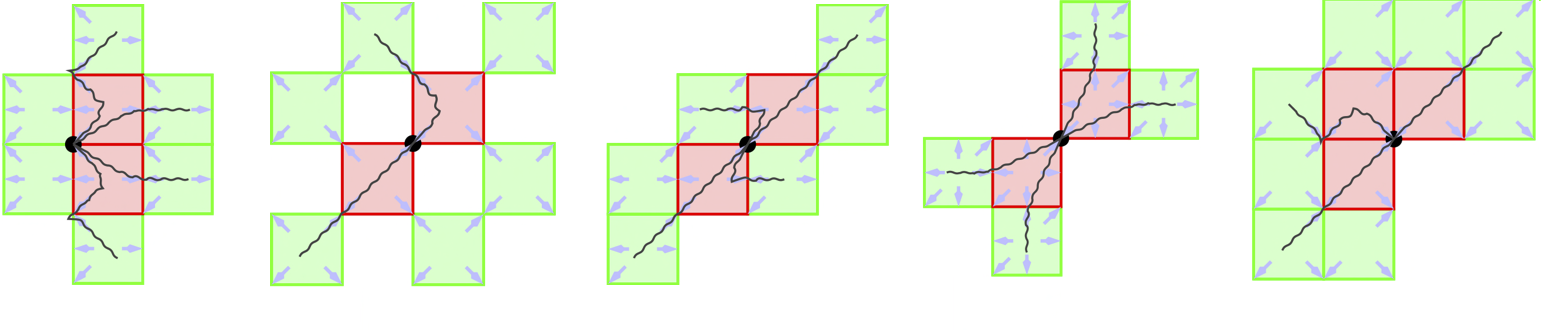
\includegraphics[width=\textwidth]{case3.png}
    \caption{Порядки угловых точек для типов {\bf A, B, C, D6, D3}.}
    \label{fig:case3}
\end{figure}

\textbf{(3)}
Пусть $x$ --- вершина для $S_\bi(P)$.
Для типов \textbf{A},  \textbf{B}, \textbf{C} и \textbf{D6} точка $x$ принадлежит не более чем двум копиям $K_\bi, K_\bj$, и в случае \textbf{D3} точка $x$ может принадлежать не болеее чем трём копиям $K_\bi, K_\bj, K_\bk$, как это показано на Рисунке \ref{fig:case3}.

Согласно Теореме \ref{thm:vertex_branching}, угловая точка $x$ имеет $Ord\leq2$ относительно каждой копии.
Более того, для типов \textbf{B} и \textbf{D3} порядок угловой точки относительно копии равен $1$.

Следовательно, для угловой точки $Ord(x,K)\leq4$ для типов {\bf A, C, D6}, $Ord(x,K)\leq3$ для типв {\bf D3} и 
$Ord(x,K)\leq2$ для типа {\bf B}.
\end{proof}



\section{Теорема о классификации фрактальных квадратов, являющихся дендритами}

\begin{proposition}\label{lem:d4bound}
Допустим $K$ относится к типу {\bf D6} и $\gamma$ --- его главное дерево.
\begin{itemize}[nolistsep]
    \item[(i)] $Ord(x,\gamma)\leq2$ для любого $x\in\dd K$;
    \item[(ii)] $Ord(x,K)\leq3$ для любого $x\in\ga$.
\end{itemize}
  

\end{proposition}

\begin{proof}
(i). Для угловых точек в $K$ неравенство $Ord(x,\gamma)\leq2$ следует из Предложения \ref{thm:corner}.

Для неугловой точки $x\in\dd K$ из доказательства Теоремы \ref{order} следует, что порядок ветвления $x$ относительно $\ga$ меньше или равно числу соседей у копии $K_i$. 
На Рисунке \ref{fig:case2} видно, что у любой копии $K_i$, отмеченной на этом Рисунке красным цветом, может быть не более двух соседей, в противном случае возникают запрещённые комбинации. 
Таким образом, $Ord(x,\gamma)\leq Ord(x,K)\leq2$.

\begin{figure}[H]
    \centering
    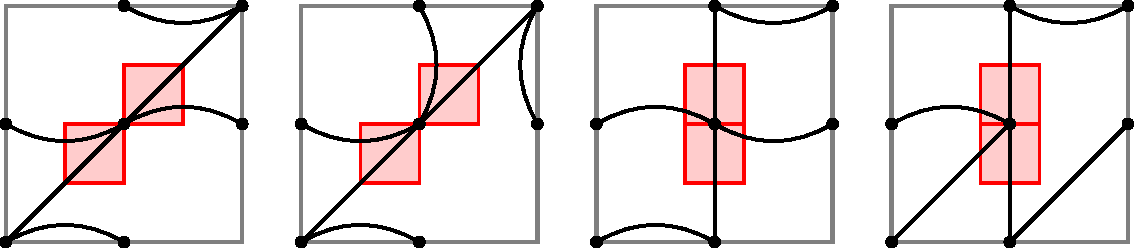
\includegraphics[width=\textwidth]{d6ord3full.pdf}
    \caption{ 
        Предполагаемые расположения главного дерева $\ga$ при допущении того, что $Ord(x,\gamma)=4$ для типа {\bf D6}. Точка $x$ располагается в центре.}
    \label{fig:d6ord3full}
\end{figure}

(ii)  Пусть существует $x\in\ga$ такое, что $Ord(x,\gamma)=4.$
Из Теоремы \ref{order} следует, что  $x=S_i(K)\cap S_j(K)$ для некоторых $i,j\in I$.\\
Рассмотрим сначала случай, когда $x$ является общей угловой точкой копий  $S_i(K)$ и $S_j(K)$, так что $x=S_i(b)=S_j(a)$, где $a=(0,0)$ и $b=(1,1)$. 
Так же обозначим $F_{0,-1}=\{c\}$, $F_{0,1}=\{d\}$, $F_{-1,0}=\{e\}$, $F_{1,0}=\{f\}$.

\begin{figure}[H]
    \centering 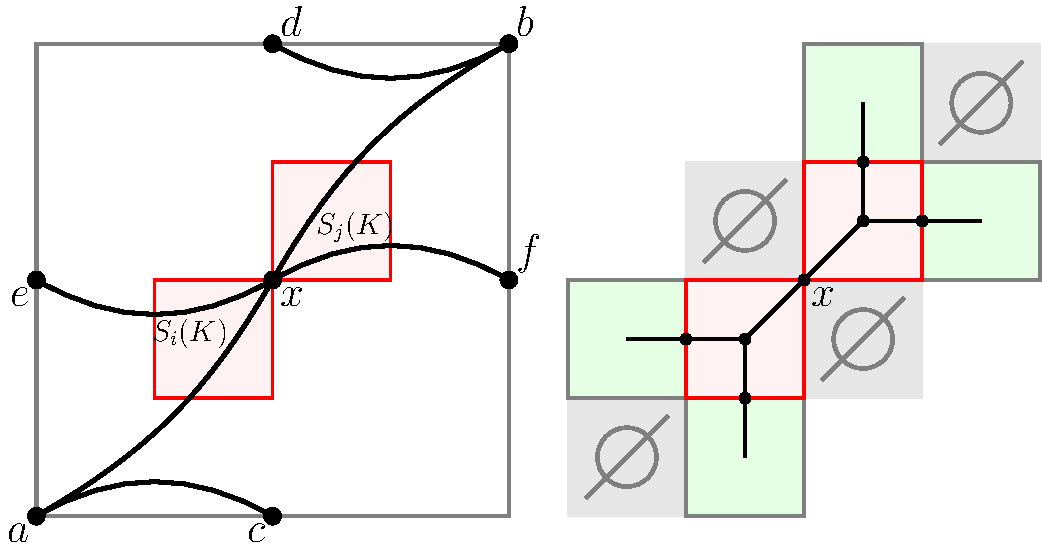
\includegraphics[width=0.8\textwidth]{d6ord3_12.pdf}
    % \caption{Caption}
    % \label{fig:d6ord3_12}
\end{figure}

Для точек $a,b$ согласно Теоремам \ref{thm:vertex_branching} и \ref{order} следует, что $Ord(a,\ga)=Ord(b,\ga)=2$. 
Значит множество $\ga\mmm\{a,b\}$ состоит из трёх компонент. 
Обозначим замыкания этих компонент как $\ga_0$, $\ga_a$, $\ga_b$ так, чтобы $\ga_0\cap\ga_a=\{a\}$ и $\ga_0\cap \ga_b=\{b\}$. 
Компонента $\ga_0$ содержит дугу $\ga(a,b)$, которая делит $P$ на две части. 
В одной из них находятся точки $c$ и $f$, в другой --- $e$ и $d$, значит $x\in \ga(a,b)$ и множество $\ga_0$ содержит одну из пар точек: $\{c,d\}$, $\{c,f\}$, $\{e,f\}$ или $\{e,d\}$.

Рассмотрим случай, когда $\ga_0\NI\{e,f\}$. 
Тогда $\ga_a=\ga(a,c)$ и $\ga_b=\ga(b,d)$.

Значит множество $\ga_0$ является объединением поддуг $\ga(a,x)$, $\ga(f,x)$, $\ga(b,x)$ и $\ga(e,x)$.

Эти четыре поддуги пересекают множество $S_i(\dd K)\cup S_j(\dd K)$ в четырёх различных точках $S_i(c)$, $S_i(e)$, $S_j(f)$, $S_j(d)$. 
поэтому пересечение этих поддуг с $S_i( K)\cup S_j(K)$ должны быть различными поддугами $S_i(\ga(c,b))$,  $S_i(\ga(e,b))$, $S_j(\ga(f,a))$, $S_j(\ga(d))$ чьи внутренности лежат в разных компонентах множества $\ga_0\mmm\{x\}$. 
Это невозможно, так как $\ga(a,f)\cap\ga(a,d)=\ga(a,x)$.\\

Рассмотрим теперь случай, когда $x$ лежит на общей стороне двух копий $S_i(K)$ и $S_j(K)$. 
В этом случае $F_{0,-1}=\{c\}$, $F_{0,1}=\{d\}$, так что $x=S_i(d)=S_j(c)$.  
Обозначим $F_{-1,-1}=\{a\}$, $F_{1 ,1}=\{b\}$, $F_{-1,0}=\{e\}$, $F_{1,0}=\{f\}$.

Для точек $c,d$ из Теоремы \ref{thm:vertex_branching}, \ref{order} следует, что $Ord(c,\ga)=Ord(d,\ga)=2$. 

Значит множество $\ga\mmm\{c,d\}$  состоит из трёх компонент. 
Обозначим замыкания эти компонент как $\ga_0$, $\ga_c$, $\ga_d$ так, чтобы $\ga_0\cap\ga_c=\{c\}$ и $\ga_0\cap \ga_d=\{d\}$. 
Компонента $\ga_0$ содержит дугу $\ga(c,d)$, которая делит $P$ на две части. 
Одна из этих частей содержит точки $b$ и $f$, другая содержит $e$ и $a$, следовательно $x\in \ga(c,d)$, а множество $\ga_0$ содержит одну из пар точек: $\{a,b\}$, $\{a,e\}$, $\{e,f\}$ или $\{b,f\}$. 

\begin{figure}[H]
    \centering
    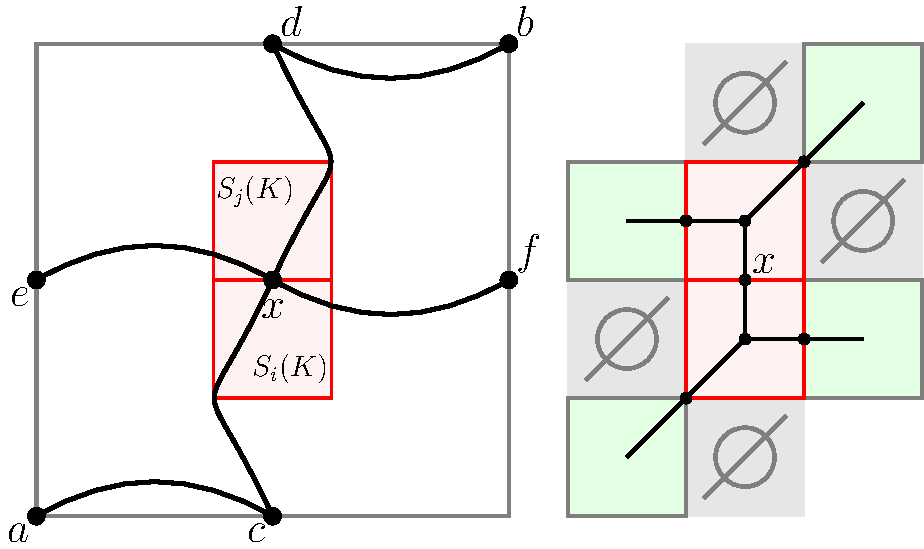
\includegraphics[width=0.8\textwidth]{d6ord3_34.pdf}
    % \caption{Caption}
    % \label{fig:d6ord3_34}
\end{figure}

Рассмотрим случай, когда $\ga_0\NI\{e,f\}$. 
Тогда $\ga_c=\ga(a,c)$ и $\ga_d=\ga(b,d)$.

Значит множество $\ga_0$ является объединением поддуг  $\ga(c,x)$, $\ga(f,x)$, $\ga(d,x)$ и $\ga(e,x)$.

Эти четыре поддуги пересекают множество $S_i(\dd K)\cup S_j(\dd K)$ в четырёх различных точках: $S_i(e)$, $S_i(b)$, $S_j(f)$ и $S_j(a)$. 
Значит пересечения этих четырёх поддуг с $S_i( K)\cup S_j(K)$ должны быть различными поддугами $S_j(\ga(c,b))$, $S_j(\ga(c,e))$, $S_i(\ga(a,d))$ и $S_j(\ga(d,f))$, внутренности которых лежат в разных компонентах множества $\ga_0\mmm\{x\}$. 
Это невозможно, так как $\ga(a,d)\cap\ga(d,f)=\ga(d,x)$.
\end{proof}

\begin{theorem}\label{thm:7trees}
Для фрактальных квадратов, являющихся дендритами, существует только $7$ топологических типов главного дерева, модели которых показаны ниже.
\end{theorem}

\begin{figure}[H]
    \centering \Large {\bf
    1. 
\includegraphics[width=0.15\textwidth]{mt1.pdf}
    \hfill
    2. 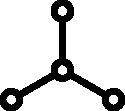
\includegraphics[width=0.15\textwidth]{mt2.pdf}
    \hfill
    3. 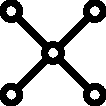
\includegraphics[width=0.13\textwidth]{mt3.pdf}
    \hfill
    4. 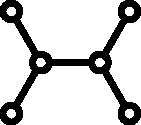
\includegraphics[width=0.15\textwidth]{mt4.pdf}\\
    \bigskip
    5. 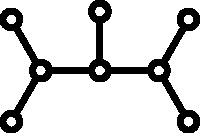
\includegraphics[width=0.23\textwidth]{mt5.pdf}
    \hfill
    6. 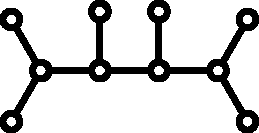
\includegraphics[width=0.3\textwidth]{mt7.pdf}
    \hfill
    7. 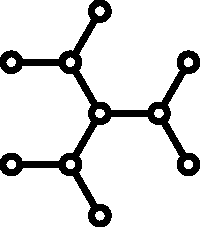
\includegraphics[width=0.22\textwidth]{mt6.pdf}}
    \caption{Семь типов главного дерева}
    \label{fig:7trees}
\end{figure}

% % \begin{figure}[H]
% %     \centering
% %     % \includestandalone[width=0.7\textwidth]{case2}
% %     \caption{Дендриты классов \textbf{(A)}, \textbf{(B)}, \textbf{(C)}, \textbf{(D3)} и \textbf{(D6)}}
% %     \label{img:dentypes}
% % \end{figure}


\begin{proof}
Пусть $K$ --- фрактальный квадрат, являющийся дендритом, с главным деревом $\ga$. 
Все концы этого дерева лежат в $\dd K$.

Пусть $K$ относится к типам {\bf A} или {\bf C}. 
Тогда, по Теореме \ref{ssboundary}, главное $\gamma$ может содержать 2, 3 или 4 конца, что соответствует моделям 1, 2, 3 и 4 на Рисунке \ref{fig:7trees}.


Если $K$ относится к типу {\bf B},то по Теоремам \ref{ssboundary} и \ref{thm:corner} главное дерево имеет ровно четыре конца, что соответствует моделям 3 и 4.

Если $K$ соответсвует типу {\bf D3}, то по Теоремам \ref{ssboundary} и \ref{thm:corner} главное дерево $\gamma$ имеет только 3 конца, что соответствует модели 2.

Если $K$ относится к типу {\bf D6}, то по Теореме \ref{ssboundary} и Лемме \ref{lem:d4bound} главное дерево $\gamma$ может иметь от 2 до 6 концов, и для любого  $x\in \gamma $ верно $ Ord(x,\gamma)\leq3$, значит $\gamma$ не может иметь форму, отличную от моделей 1, 2, 4, 5, 6 или 7 с Рисунка \ref{fig:7trees}.
\end{proof}

\begin{remark}
Если $K$ относится к типу {\bf D6}, то его главное дерево $\gamma$ не может иметь форму, отличную от моделей 4, 5, 6 или 7 с Рисунка \ref{fig:7trees}.
Невозможность моделей 1 и 2 главного дерева фрактальных квадратов типа {\bf D6} обусловлена тем, что число концов в $\gamma$ для типа {\bf D6} не меньше 4.
Однако для доказательства Теоремы \label{thm:7trees} это не требуется.
\end{remark}

Таким образом, если мы будем классифицировать фрактальные квадраты, являющиеся дендритами, по форме главного дерева, то мы получим 7 классов фрактальных квадратов.
Такую классификацию мы можем называть {\em общей классификацией} или {\em классификацией по форме главного дерева}.

Если принять во внимание гипотезу о том, что во фактальном квадрате типа {\bf D6} число концов в его главном дереве $\gamma$ не меньше 4, то мы можем рассмотеть {\em тонкую классификацию}, учитывающую следующие признаки:
\begin{itemize}[nolistsep]
	\item[1.] форма главного дерева (1 из 7 типов);
	\item[2.] тип самоподобной границы ({\bf A}, {\bf B}, {\bf C}, {\bf D3} или {\bf D6});
	\item[3.] порядки ветвления точек самоподобной границы в главном дереве.
\end{itemize}

Примеры фрактальных квадратов из каждого класса тонкой классификации показаны на следующих рисунках.
Всего получается 16 классов.
Отдельно стоит сказать, что классы 3 ({\bf 2-A-1}) и 4 ({\bf 2-A-2}) с Рисунка \ref{fig:tree2} имеют одинаковый тип дерева и одинаковый тип самоподобной границей, но отличаются порядком ветвления точек самоподобной границы в главном дереве: в {\bf 2-A-1} три конца и одна разбивающая точка, а в {\bf 2-A-2} три конца и одна точка ветвления порядка 3.
Это единсвенные два класса, которые различаются только по третьему признаку.


\begin{figure}[H]
    \centering
    
\includegraphics[scale=1.5]{mt1.pdf}
    \vspace{0.5cm}
    \vfill
    \fbox{
    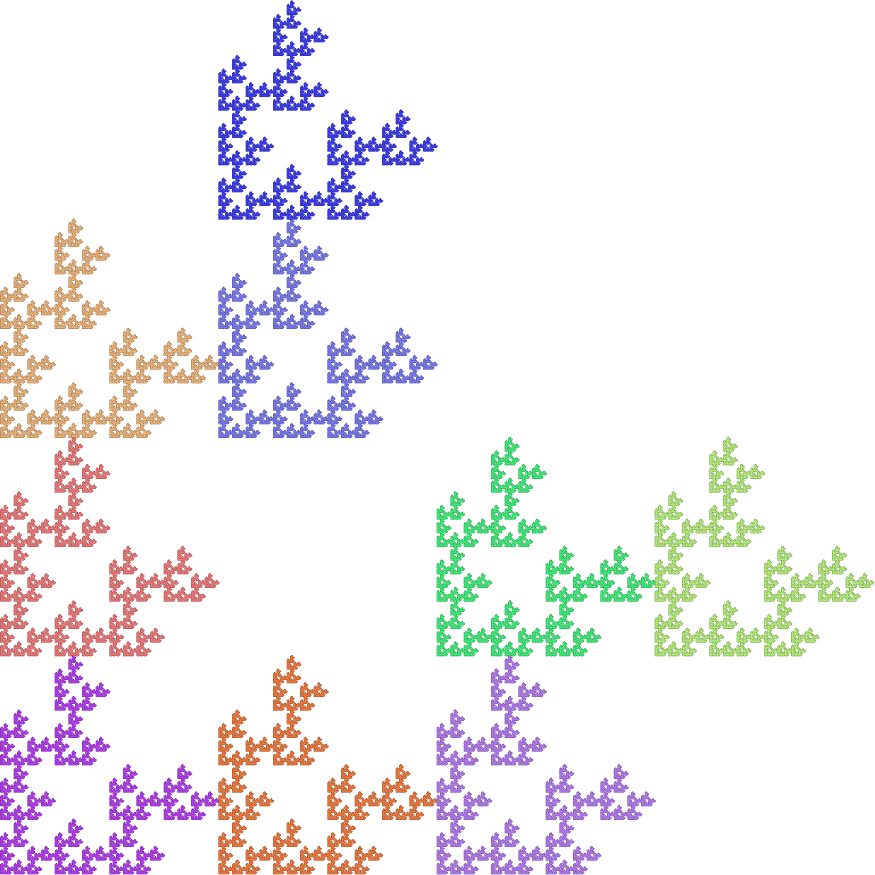
\includegraphics[width=0.22\textwidth]{1K.png}
    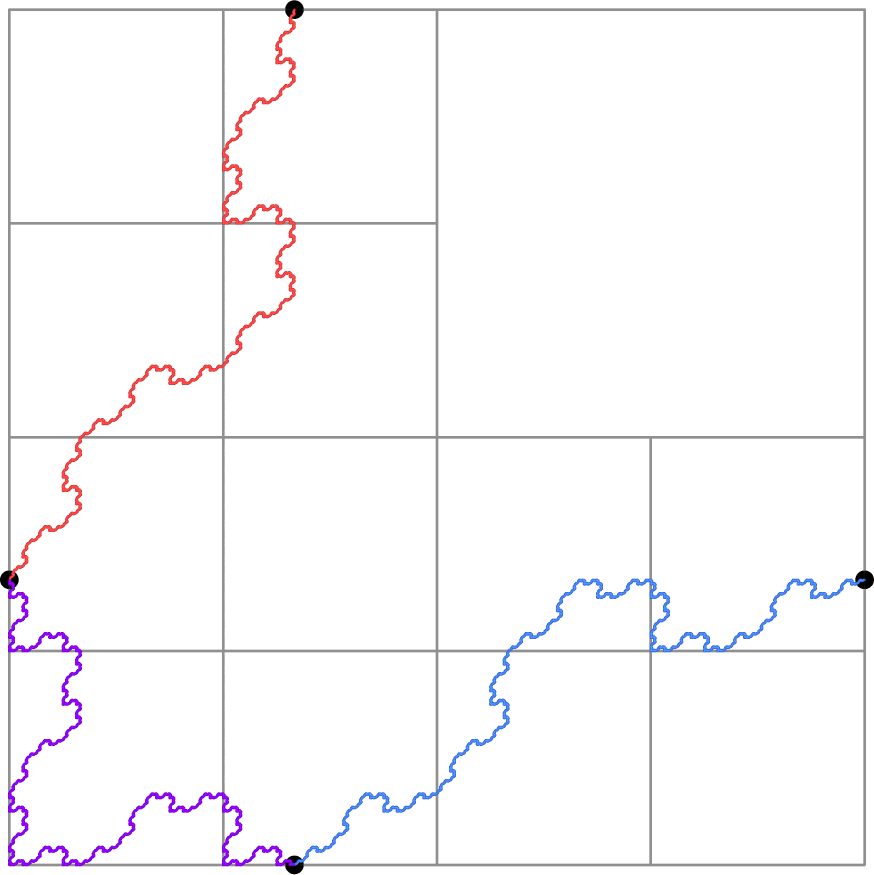
\includegraphics[width=0.22\textwidth]{1T.png}}
    \hfill
    \fbox{
    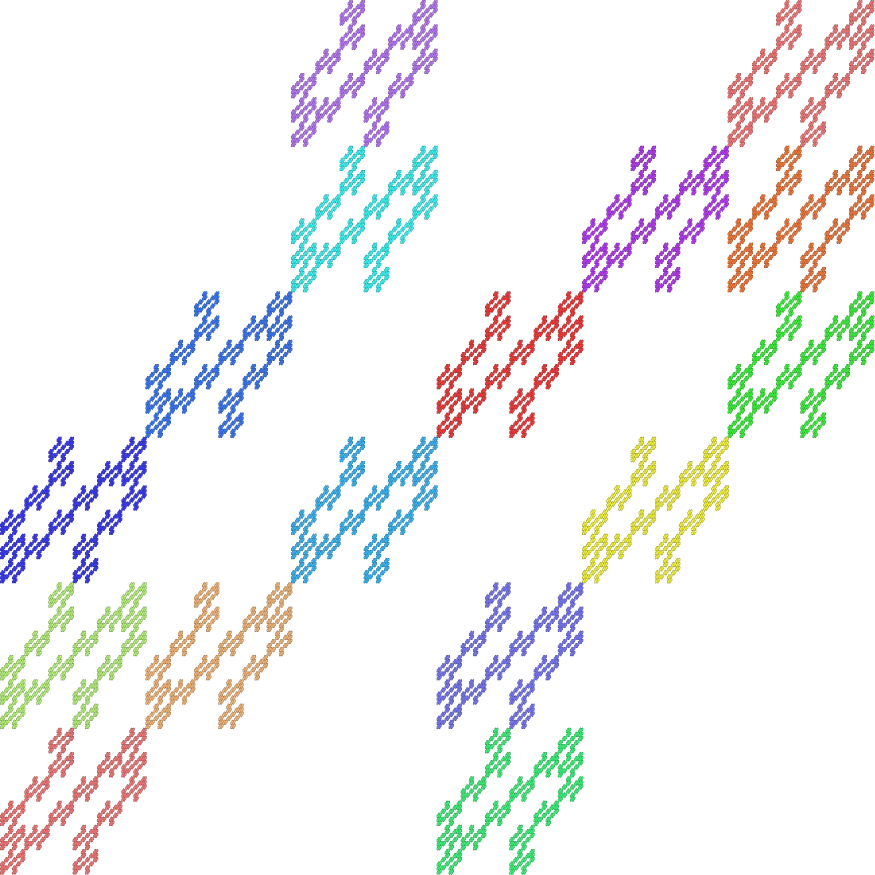
\includegraphics[width=0.22\textwidth]{2K.png}
    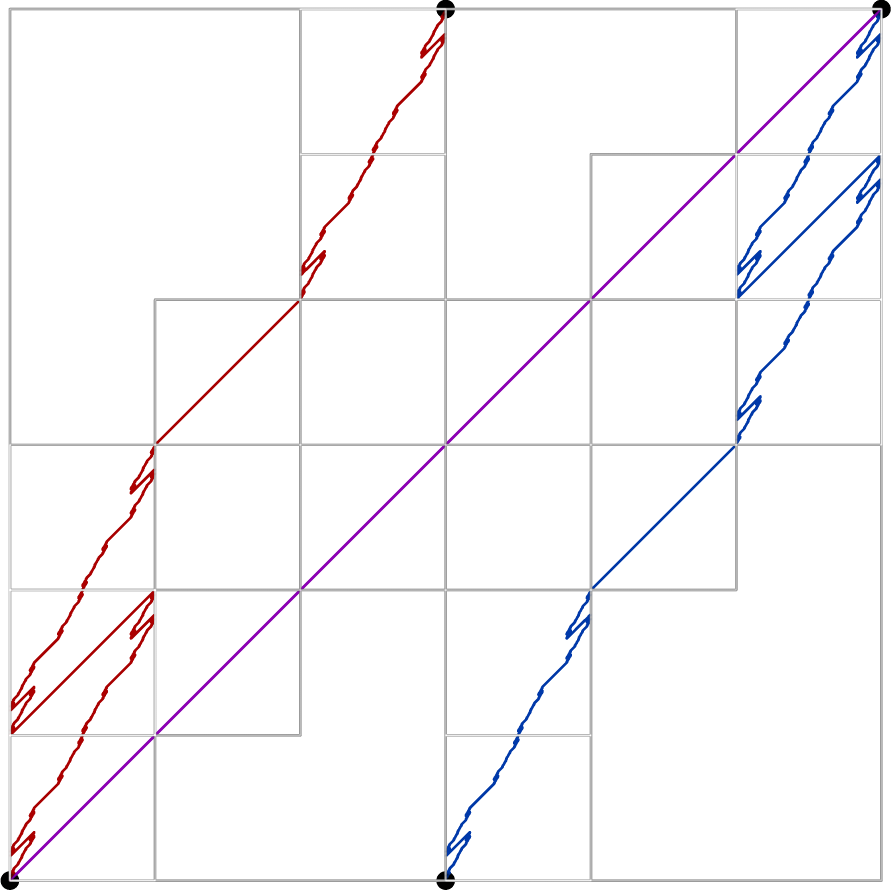
\includegraphics[width=0.22\textwidth]{2T.png}}
    \caption{Дерево 1. Классы 1 и 2 (обозначим как \textbf{1-A} и \textbf{1-C}). }
    \label{fig:tree1}
\end{figure}

\begin{figure}[H]
    \centering
    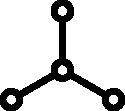
\includegraphics[scale=1.5]{mt2.pdf}
    \vspace{0.5cm}\vfill
    \fbox{
    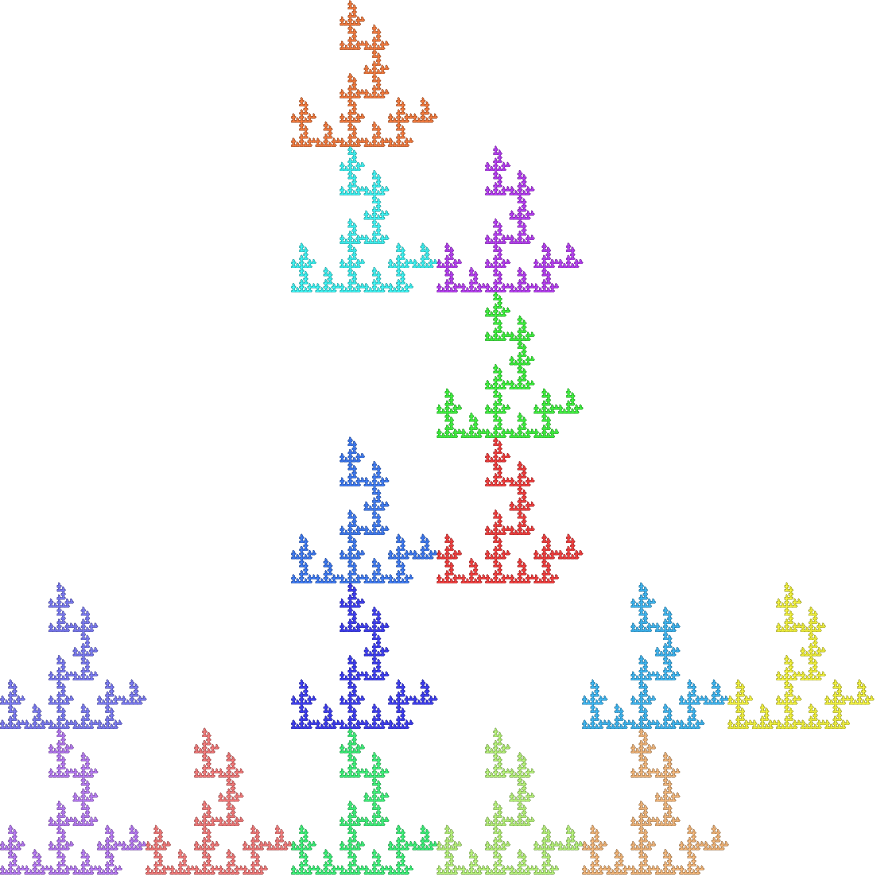
\includegraphics[width=0.22\textwidth]{3K.png}
    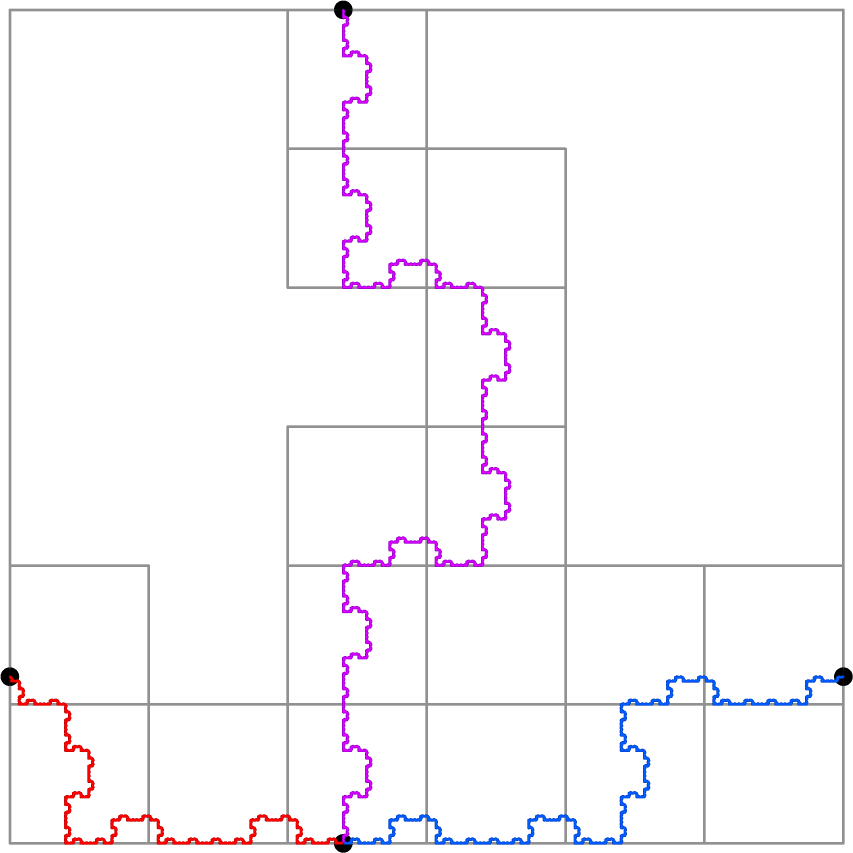
\includegraphics[width=0.22\textwidth]{3T.png}}
    \hfill
    \fbox{
    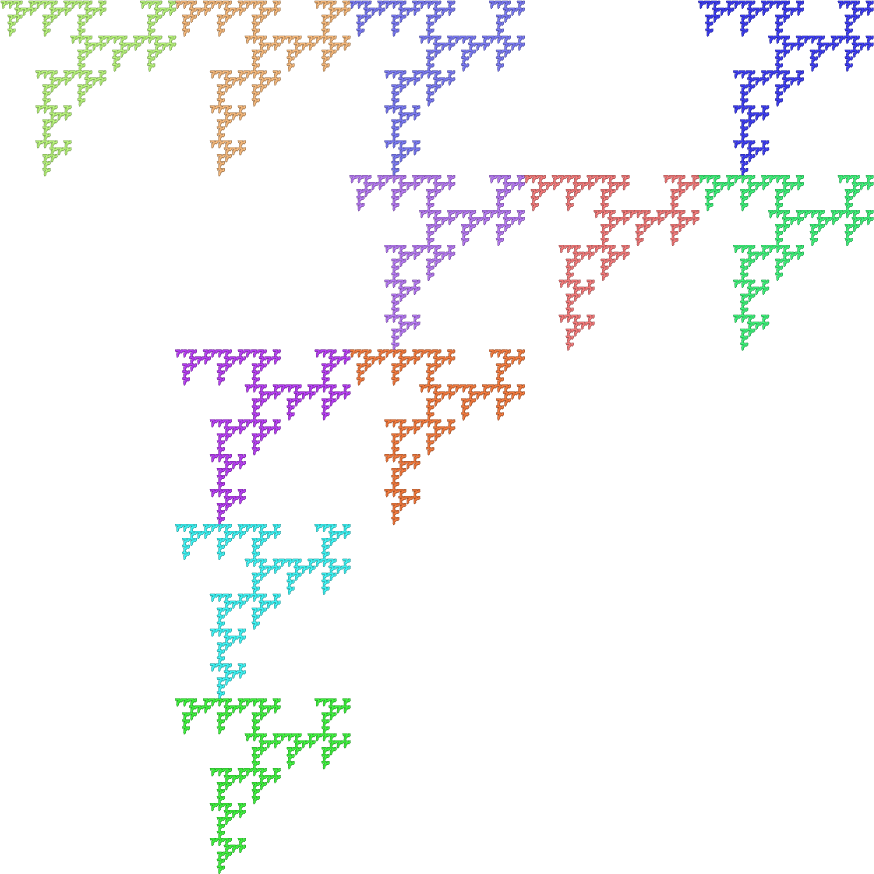
\includegraphics[width=0.22\textwidth]{4K.png}
    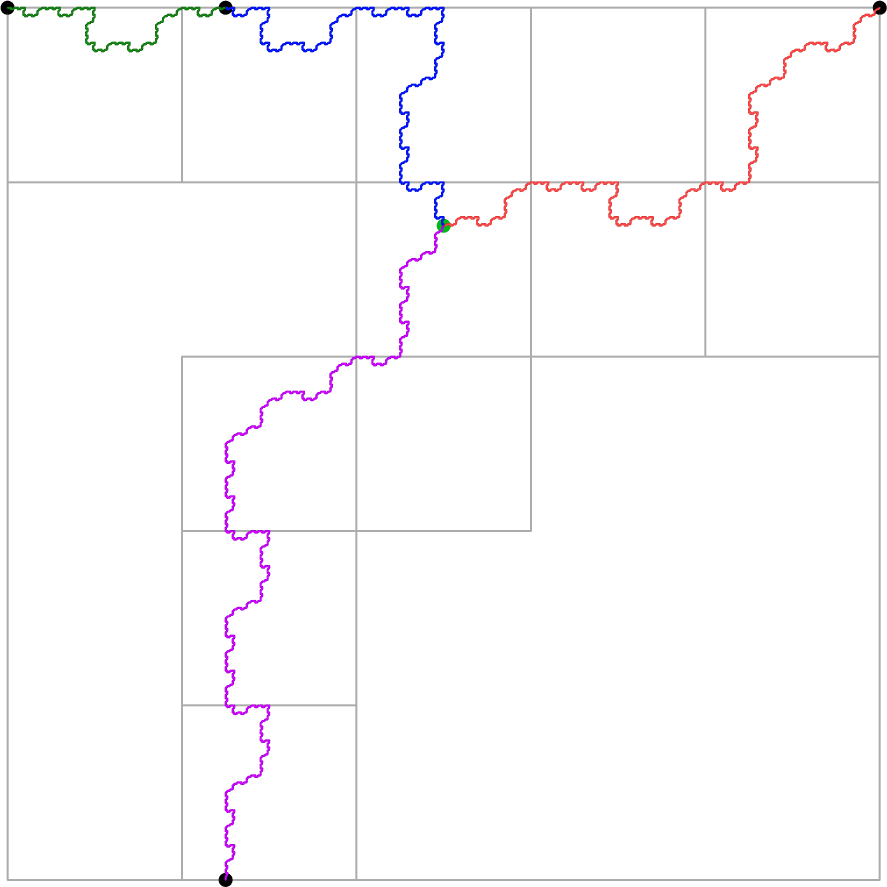
\includegraphics[width=0.22\textwidth]{4T.png}}
    \vspace{0.3cm}\vfill
    \fbox{
    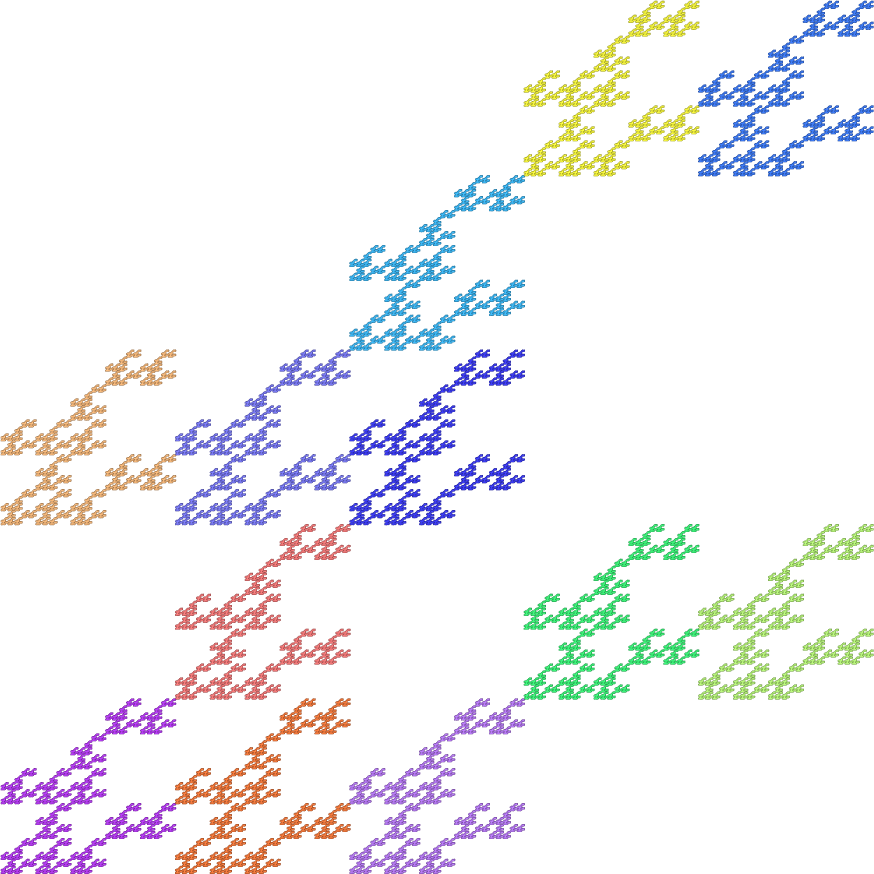
\includegraphics[width=0.22\textwidth]{5K.png}
    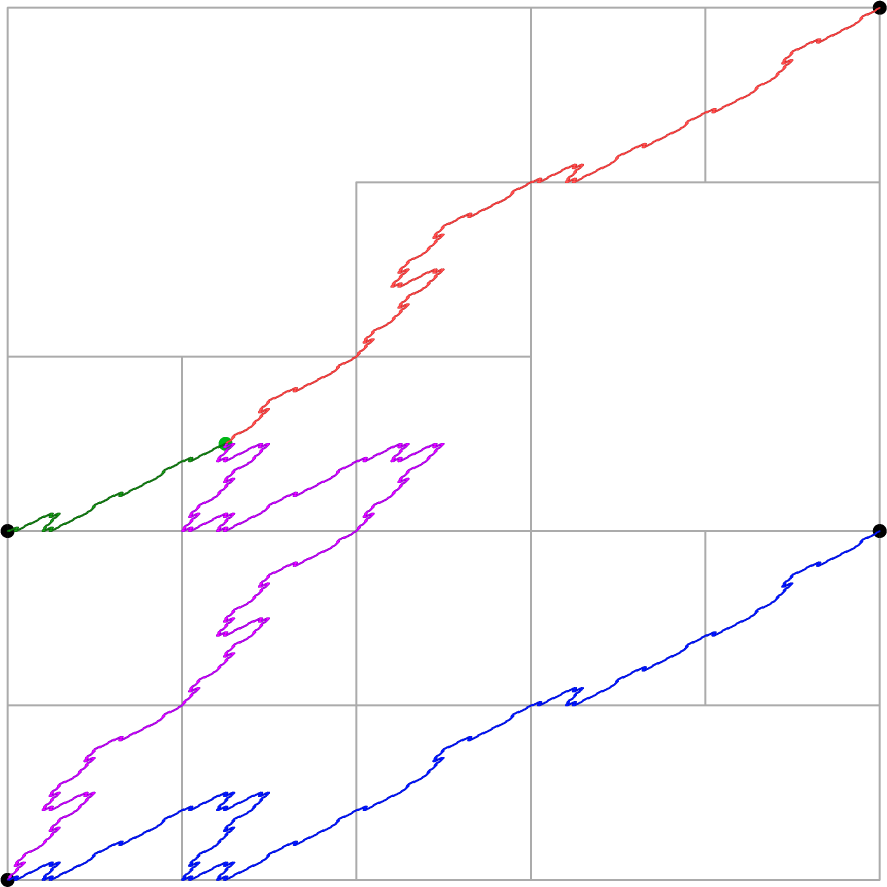
\includegraphics[width=0.22\textwidth]{5T.png}}
    \hfill
    \fbox{
    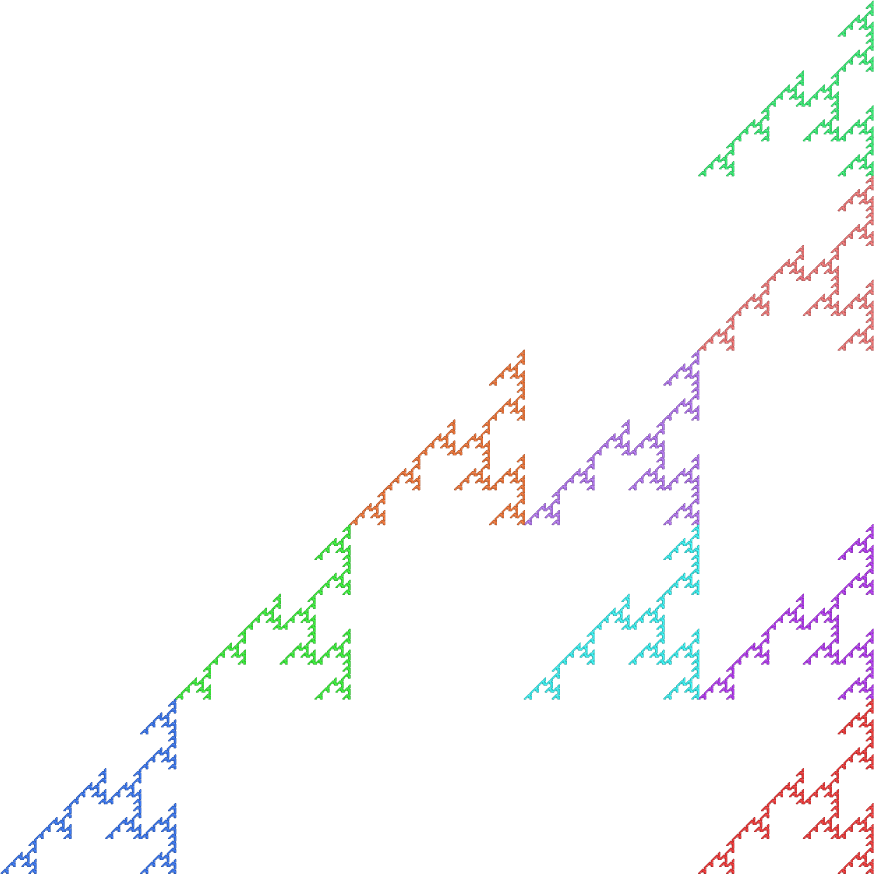
\includegraphics[width=0.22\textwidth]{6K.png}
    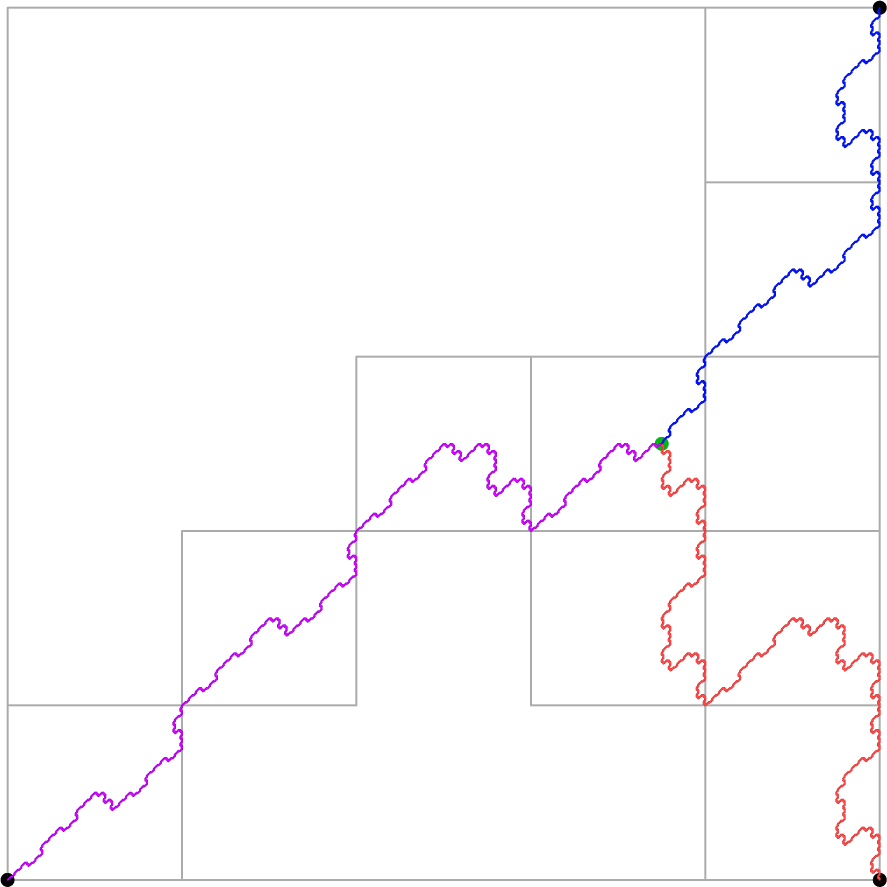
\includegraphics[width=0.22\textwidth]{6T.png}}
    \caption{Дерево 2. Классы 3 ({\bf 2-A-1}), 4 ({\bf 2-A-2}), 5 ({\bf 2-D6}) и 6 ({\bf 2-D3})}
    \label{fig:tree2}
\end{figure}

\begin{figure}[H]
    \centering
    \hspace{0.12\textwidth}
    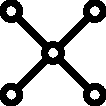
\includegraphics[scale=1.5]{mt3.pdf}
    \hfill
    \fbox{
    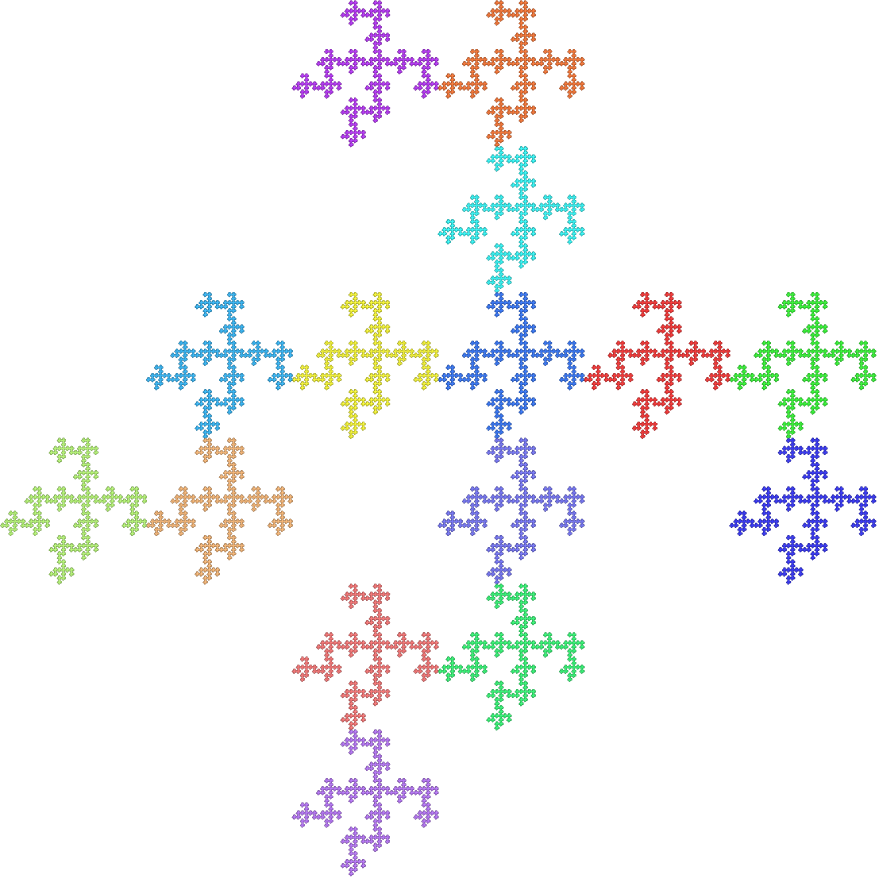
\includegraphics[width=0.22\textwidth]{7K.png}
    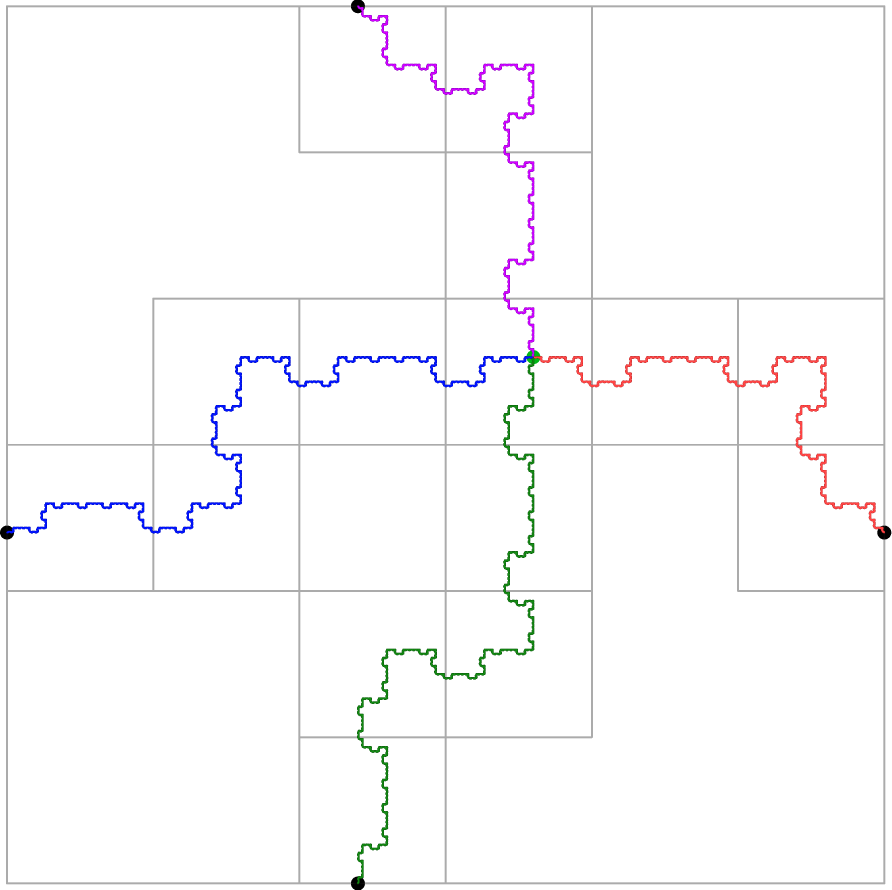
\includegraphics[width=0.22\textwidth]{7T.png}}
    \vspace{0.3cm}\vfill
    \fbox{
    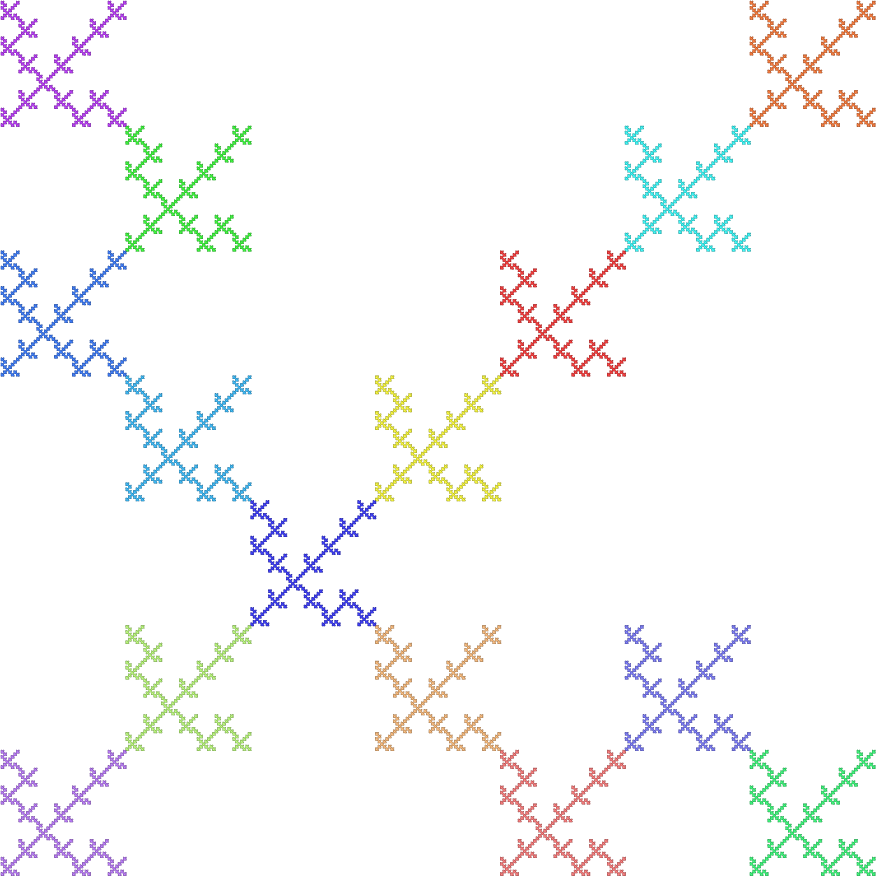
\includegraphics[width=0.22\textwidth]{8K.png}
    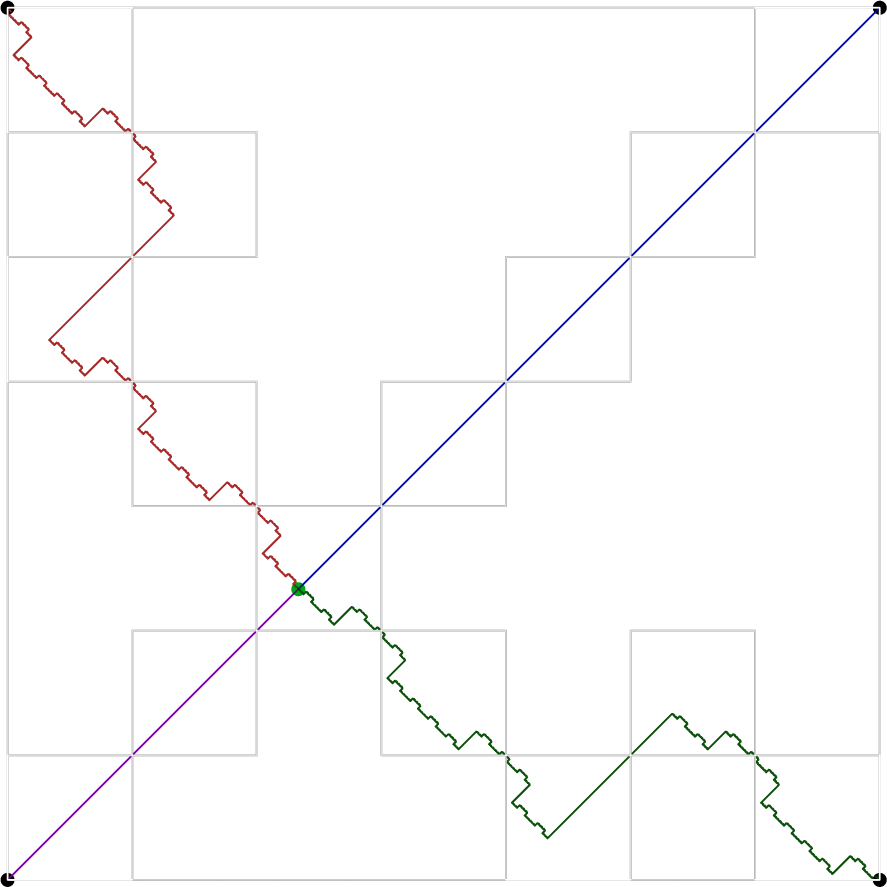
\includegraphics[width=0.22\textwidth]{8T.png}}
    \hfill
    \fbox{
    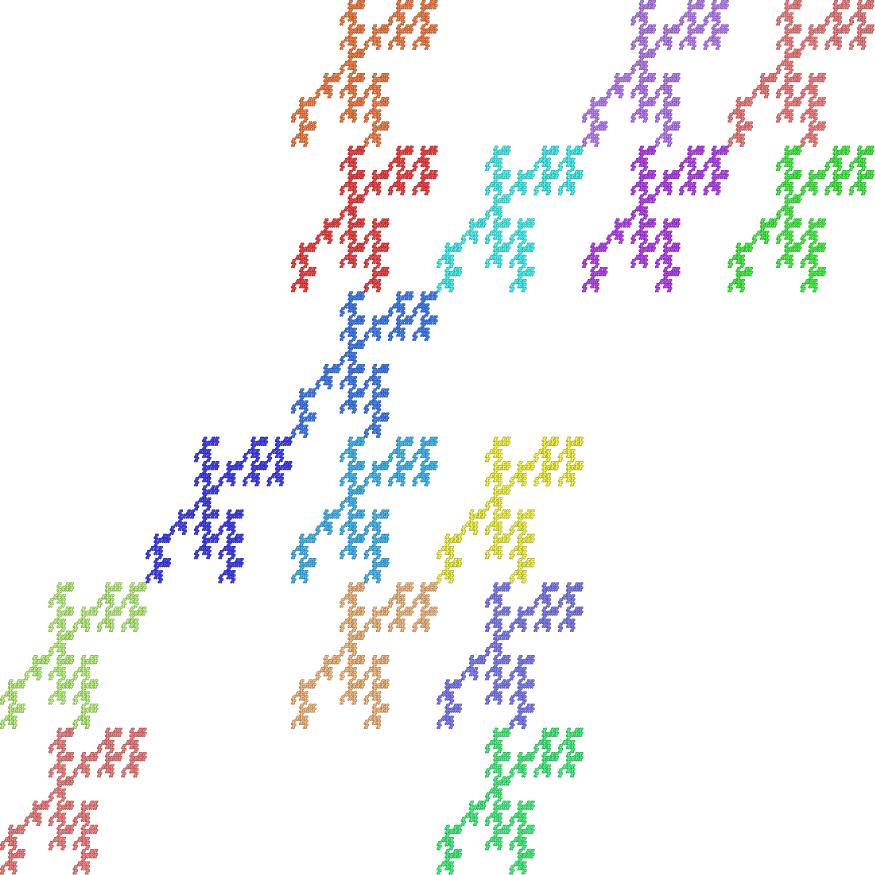
\includegraphics[width=0.22\textwidth]{9K.png}
    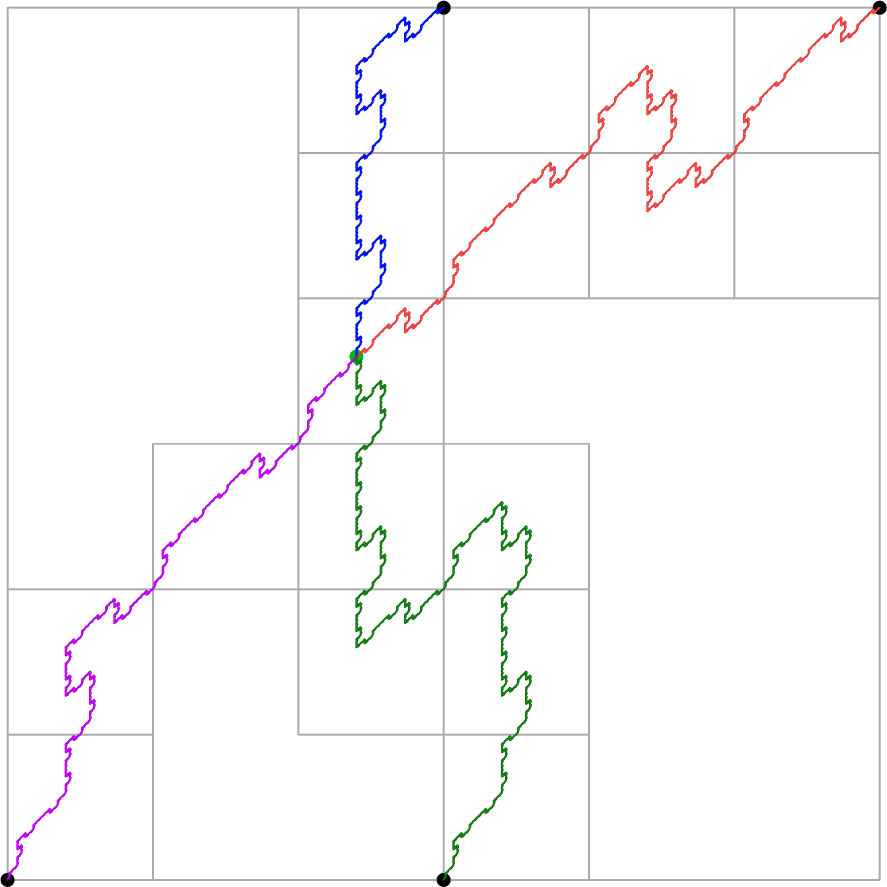
\includegraphics[width=0.22\textwidth]{9T.png}}
    \caption{Дерево 3. Класс 7 ({\bf 3-A}), 8 ({\bf 3-B}) и 9({\bf 3-C})}
    \label{fig:tree3}
\end{figure}
 
\begin{figure}[H]
    \centering
    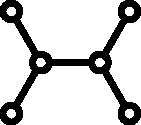
\includegraphics[scale=1.5]{mt4.pdf}
    \vspace{0.5cm}\vfill
    \fbox{
    \includegraphics[width=0.22\textwidth]{10K.png}
    \includegraphics[width=0.22\textwidth]{10T.png}}
    \hfill
    \fbox{
    \includegraphics[width=0.22\textwidth]{11K.png}
    \includegraphics[width=0.22\textwidth]{11T.png}}
    \vspace{0.3cm}\vfill
    \fbox{
    \includegraphics[width=0.22\textwidth]{12K.png}
    \includegraphics[width=0.22\textwidth]{12T.png}}
    \hfill
    \fbox{
    \includegraphics[width=0.22\textwidth]{13K.png}
    \includegraphics[width=0.22\textwidth]{13T.png}}
    \caption{Дерево 4. Классы 10 ({\bf 4-A}), 11 ({\bf 4-B}), 12 ({\bf 4-C}) и 13 ({\bf 4-D6})}
    \label{fig:tree4}
\end{figure}

\begin{figure}[H]
    \centering
    \includegraphics[scale=1.4]{mt5.pdf}
    \hfill
    \fbox{
    \includegraphics[width=0.22\textwidth]{14K.png}
    \includegraphics[width=0.22\textwidth]{14T.png}}
    \caption{Дерево 5. Класс 14 ({\bf 5-D6})}
    \label{fig:tree5}
\end{figure}

\begin{figure}[H]
    \centering
    \includegraphics[scale=1.4]{mt7.pdf}
    \hfill
    \fbox{
    \includegraphics[width=0.22\textwidth]{15K.png}
    \includegraphics[width=0.22\textwidth]{15T.png}}
    \caption{Дерево 6. Класс 15 ({\bf 6-D6})}
    \label{fig:tree6}
\end{figure}

\begin{figure}[H]
    \centering
    \includegraphics[scale=1.2]{mt6.pdf}
    \hfill
    \fbox{
    \includegraphics[width=0.22\textwidth]{16K.png}
    \includegraphics[width=0.22\textwidth]{16T.png}}
    \caption{Дерево 7. Класс 16 ({\bf 7-D6})}
    \label{fig:tree7}
\end{figure}
